\documentclass[11pt]{article}
%\usepackage{epsfig}
\usepackage{graphicx}
\usepackage{amsmath}
\usepackage{amsthm}
\usepackage{amsfonts}
\usepackage{algorithm}
\usepackage{adjustbox}
\usepackage{tikz}
\usepackage{bm}
\usepackage{enumitem}
\usepackage{mathtools}

\usepackage{pgfplots} 

\newcommand{\myquote}[1]{``#1''}

\usepackage{array} %\newcommand{\PreserveBackslash}[1]{\let\temp=\\#1\let\\=\temp}
%\newcolumntype{C}[1]{>{\PreserveBackslash\centering}m{#1}}
%\newcolumntype{R}[1]{>{\PreserveBackslash\raggedleft}m{#1}}
%\newcolumntype{L}[1]{>{\PreserveBackslash\raggedright}m{#1}}

\usepackage{multirow}
\usepackage{booktabs}


\addtolength{\oddsidemargin}{-0.55in}
	\addtolength{\evensidemargin}{-0.5in}
	\addtolength{\textwidth}{1in}
	\addtolength{\textheight}{0.5in}

\newtheorem{claim}{Claim} 
\newtheorem{proposition}{Proposition} 
\newtheorem{teo}{Theorem} 
\newtheorem{corollary}{Corollary} 

%\newenvironment{proof}{\noindent {\bf Proof:} \hspace{.677em}}%
{}
\newcommand{\beq}{\begin{equation}}
\newcommand{\eeq}{\end{equation}}
\newcommand{\naturali}{\mathbb{N}}

\newcommand{\ZZ}{\mathbb{Z}}
\newcommand{\RR}{\mathbb{R}}

%\newcommand{\mod}{\textrm{mod}}
\newcommand{\opt}[1]{$#1$-OPT}
\newcommand{\kopt}{\opt{k}}
\newcommand{\pref}[1]{(\ref{#1})}
\newcommand{\edg}[2]{\{#1,#2\}}
%\newcommand{\PP}[1]{{\cal P}(#1)}
\newcommand{\PP}[1]{[#1\textrm{?}]}
\newcommand{\pzero}{{\cal Z}}
\newcommand{\ins}[2]{I(#1,#2)}  
\newcommand{\Reins}[2]{<#1,#2>}  
\newcommand{\Reinss}[3]{<#1,#2,#3>}  
\newcommand{\reins}[3]{<#1,#2,#3>}  
\newcommand{\reinss}[4]{<#1,#2,#3,#4>}

\newcommand{\COMM}[1]{[{\bf *** #1 ***}]}

\renewcommand{\rq}[1]{r_{#1}}

\newcommand{\orbit}[1]{{\cal O}(#1)}
   
\usepackage{amsmath,amsbsy}
%\newcommand*{\piu}{\ensuremath{\boldsymbol{\pmb{+}}}}
%\newcommand*{\piu}{{\ensuremath{\pmb{+}}}}

% questi:?
%\newcommand*{\meno}{\boldsymbol{\,\pmb{-}\,}}
%\newcommand*{\piu}{\pmb{+}}

\newcommand{\piu}{\oplus}
\newcommand{\meno}{\ominus}
%\newcommand{\piu}{\bm{+}}
%\newcommand{\meno}{\pmb{-}}
%\newcommand{\falpha}{\alpha}
%\newcommand{\fbeta}{\beta}
%\newcommand{\fgamma}{\gamma}
%\newcommand{\fdelta}{\delta}
%\newcommand{\ffalpha}{\alpha}
%\newcommand{\ffbeta}{\beta}
%\newcommand{\ffgamma}{\gamma}
%\newcommand{\ffdelta}{\delta}
 
   
\newcommand{\falpha}{f_r^1}
\newcommand{\fbeta}{f_r^2}
\newcommand{\fgamma}{f_r^3}
\newcommand{\fdelta}{f_r^4}
\newcommand{\ffalpha}{1}
\newcommand{\ffbeta}{2}
\newcommand{\ffgamma}{3}
\newcommand{\ffdelta}{4}

\begin{document}
	\title{Orbits, schemes and dynamic programming procedures for the TSP \opt{4}\ neighborhood %for the TSP
		} 		
		\author{Giuseppe Lancia\thanks{DMIF, Univ. of Udine, Italy} \and Marcello Dalpasso\thanks{DEI, Univ. of Padova, Italy}}
\date{}
\maketitle

\begin{abstract}
We discuss the way to group all 25 possible 4-OPT moves into 7 orbits of equivalent moves. We then describe two implementations, one for a $\Theta(n^3)$ algorithm by 
de Berg's et al. and one of a $\Theta(n^2)$ algorithm by
Glover, for finding the best 4-OPT move via dynamic
programming.
\end{abstract}

\newcommand{\bimp}{best-improving}

\section{Introduction}

In this paper we focus on the (symmetric)
Traveling Salesman Problem (TSP), i.e., the problem of finding a shortest hamiltonian cycle (a shortest {\em tour})
on a complete graph of $n$ nodes weighted on the edges.
Let us denote by $c(i,j)=c(j,i)$ the distance between any two nodes $i$ and $j$.  A tour is identified by a permutation of
vertices $(v_1,\ldots,v_n)$. We call $\{v_i, v_{i+1}\}$,  for $i=1,\ldots,n-1$, and $\{v_n,v_1\}$ the {\em edges of the tour}.
The length of a tour $T$, denoted by $c(T)$, is the sum of the lengths of the edges of the tour. More generally, for any set $F$ of edges, we denote by $c(F)$ the value $\sum_{e\in F} c(e)$.

A large number of applications over the years have shown that {\em local search} 
%, albeit one of the simplest, 
is often a very effective way to tackle hard combinatorial optimization problems \cite{PapSte,AaLe97}.
As far as the TSP is concerned, a famous and successful approach in the past
year has been local search based on the {\em \kopt\ neighborhood}, particularly for $k=2,3$.

Let $k\ge 2$ be an integer constant.
A \kopt\ move on a tour $T$ consists in first removing a set $R$ of $k$ edges and then inserting  a set $I$ of
$k$ edges  so as $(T\setminus R) \cup I$ is still a 
tour.
A \kopt\ move is {\em improving} if
$c((T\setminus R) \cup I) < c(T)$
i.e., $c(I) < c(R)$.
An improving move is {\em \bimp} if $c(R)- c(I)$ is the maximum over all possible choices of $R,I$.
The standard local search approach for the TSP based
on the \kopt\ neighborhood starts from any tour $T^0$ 
(usually a random permutation of the vertices) and then proceeds along a sequence of tours $T^1,T^2,\ldots,T^N$ where each tour $T^j$ is obtained by applying an improving \kopt\ move to $T^{j-1}$. The final tour $T^N$ is such that 
there are no improving \kopt\ moves for it.  The hope is that $T^N$ is a good tour (optimistically, a global optimum) but its quality depends on many factors. One of them is the size of the neighborhood (in this case, $\Theta(n^k)$),
%(i.e., the number of tours which can be obtained by the application of a move), 
the rationale being that with a larger-size neighborhood we sample a larger number of potential solutions, and hence increase the probability of ending up at a really good one. Clearly, there is a trade-off between the size of a neighborhood and the time required to explore it, so that most times people resort to the use of small neighborhoods since they are very fast to explore.
%(for a discussion on how to deal with some very large size, i.e., exponential, neighborhoods for various combinatorial optimization problems, see \cite{AHUJA200275}).

The first use of \kopt\ dates back to 1958 with the introduction of \opt{2}  in \cite{Croes2opt}.
In 1965  Lin \cite{Lin65} described the  \opt{3} neighborhood, and experimented with a complete enumeration algorithm, of complexity $\Theta(n^3)$, which finds the best \opt{3} move by trying all possibilities. He also introduced a heuristic step fixing some edges of the solution (at risk of being wrong) with the goal of increasing the size of the instances. Still the instances which could be tackled at the time were fairly small ($n\le 150$). Later in 1968, Steiglitz and Weiner \cite{SW} described
an improvement over Lin's method which made it 2 or 3 times faster (although still cubic).

In this paper we focus on the \opt{4} neighborhood, since, in a follow-up work, we are going to describe an effective way for determining the best \opt{4} move, based on a similar approach than the one we followed for exploring the \opt{3} neighborhood \cite{LD20}.

A \opt{4} move starts by removing four edges from a tour, thus creating four separate paths. Then it inserts four edges in such a way as to reconnect the paths into a full tour. There are 25 ways to do so, as we will show later in the paper, so that, basically, there are 25  different types of possible \opt{4} moves. However, many of these moves can be considered equivalent, in the sense that they \myquote{follow the same pattern} (this statement will be made clear later on).
In order to simplify the description of \opt{4} search algorithms, we then formally describe,
in Section \ref{sec:sele}, the equivalence between 
some different moves, and reduce the number of cases to 
consider from 25 to in fact just 7.

In the second part of the paper, we address two algorithms from the literature on the \opt{4} neighborhood. In particular, de Berg et al.
\cite{woeginger} have described a dynamic programming procedure to find the best \opt{4} move in time $\Theta(n^3)$. 
In another paper, Glover \cite{Glover1996} has described a $\Theta(n^2)$ algorithm for finding the best \opt{4} move, but valid only for three particular types of \opt{4} moves. 

The original papers \cite{woeginger,Glover1996} are
not easy reads, and the description of the algorithms can,
in our opinion, be made simpler via the description of dynamic programming relations, which correspond to algorithms of exactly the same complexity as the original versions.
In  Section \ref{sec:literature}, we then describe these dynamic programs, for de Berg et al. and Glover's algorithms.



\section{Selections, schemes and moves}
\label{sec:sele}

Let $G=(V,E)$ be a complete graph on $n$ nodes, and $c:E\mapsto \mathbb{R}^+$ be a cost function for the edges. Without loss of
generality, we assume $V=\{0,1,\ldots,\bar n\}$, where 
$\bar n:=n-1$.  
% In this paper we will describe an effective strategy for findingeither the best improving or any improving move for  a given current tour $(v_1,\ldots,v_n)$.
Furthermore, we always assume the current tour to be the tour $0\rightarrow 1 \rightarrow \cdots \rightarrow \bar n\rightarrow 0$.

We will be using modular arithmetic frequently. For convenience, for each $x\in V$ and $t\in\naturali$ we define
\[
x \piu t := (x + t) \mod n,  \qquad \textrm{} \qquad  x \meno t := (x - t) \mod n.
\]
%A tour is a permutation of vertices $(v_1,\ldots,v_n)$.  W.l.o.g. we stipulate that each tour starts with $v_1=0$.
When moving from $x$ to $x\piu 1, x\piu 2$ etc. we say that we are moving clockwise, or forward. In going from $x$ to $x\meno 1,x\meno 2,\ldots$ we say that we are moving counter-clockwise, or backward.

%%%% non mi pare sia usata--- la rimuovo
%We define the {\em forward distance} $d^-(x,y)$ from  node $x$ to node $y$ as the unique $t\in \{0,\ldots, n-1\}$ such that $x\piu t = y$.
%Similarly, we define the {\em backward distance} $d^-(x,y)$ from $x$ to $y$  as the  $t\in \{0,\ldots, n-1\}$ such that $x\meno t = y$.
%Finally, the {\em distance}  between any two nodes $x$ and $y$ is defined by
%\[
%d(x,y):= \min\{d^+(x,y), d^-(x,y)\}.
%\]

\newcommand{\selection}{{\cal S}}


A \opt{4}\ move is fully specified by two sets, i.e., the set of
removed and of inserted edges. 
We call a {\em removal set} any set of four tour edges, i.e., four edges of type $\edg{i}{i\piu 1}$. A removal set is identified by a  quadruple $S=(i_1,i_2,i_3,i_4)$ with $0 \le i_1 < i_2  < i_3 < i_4 \le \bar n$, where the edges removed are $R(S):=\{\edg{i_j}{i_j \piu 1} : j=1,\ldots,4\}$. We call any such quadruple $S$ a {\em selection}.
A selection is {\em complete} if
$i_{h}\piu 1\notin\{i_1,\ldots,i_4\}$ for each $h=1,\ldots,4$ (i.e., if the move never removes two consecutive edges of the tour), otherwise we say that $S$ is a {\em partial} selection. % We denote  the set of all complete selections by $\selection$.
Complete selections should be distinguished from partial \opt{4}  selections, since the number of choices required to determine a partial selection is actually lower than 
four. For instance, there is only a cubic number of selections in which $i_4=i_3\piu 1$ since we can choose $i_1$, $i_2$ and $i_3$ but the value of $i_4$ is forced. 


\newcommand{\reinsset}{{\cal I}}

Let $S$ be a selection and $I\subset E$ with $|I|=4$. If $(T \setminus R(S)) \cup I$ is still a tour then $I$ is called a {\em  reinsertion set}. 
Given a selection $S$, a reinsertion set $I$ is {\em pure} if $I\cap R(S) = \emptyset$, and {\em degenerate} otherwise. 
Finding the best \opt{4}\ move when the reinsertions are constrained to be degenerate is $O(n^3)$ (in fact, \opt{4} degenerates to either \opt{2} or \opt{3} in this case). Therefore, the most computationally expensive task is to determine the best move when {\em the selection is complete and the reinsertion is pure}.
We  refer to this kind of moves as {\em true} \opt{4}. 
Thus, in the remainder of the paper we will focus on true  \opt{4}\ moves.


 \subsection{Symmetries and orbits of reinsertion sets}

Let $\selection$ be the set of all complete selections. 
For $S\in \selection$, let us denote by $\reinsset(S)$ the set of all
pure reinsertion sets for $S$. 
Then, the set of all true \opt{4}\ moves is
\beq
\big\{\big(R(S),I\big) : S\in \selection, I\in \reinsset(S)\big\}
\label{set:allmoves}
\eeq
and the total number of true \opt{4} moves is
%\beq
$\sum_{S\in\selection} |\reinsset(S)| = \gamma \,|\selection|$,
%\label{eq:countmoves}
%\eeq
where  $\gamma$
specifies in how many different ways a tour can be reassembled back after four edges have been removed and replaced by four different ones.
We will see in section \ref{sec:comb} that this number, a constant over all the selections $S$, equals $25$ for \opt{4}.

According to \pref{set:allmoves}, to list all true \opt{4}\ moves we could consider a case analysis in which we go through all pure reinsertion sets for all complete selections. We can, however, simplify this case analysis by grouping together different reinsertion sets which are, in fact, equivalent. 

To define the equivalence between reinsertion sets, let us introduce a standard way to draw a tour with a reinsertion set. This type of figures will be in 1-to-1 correspondence with the reinsertion sets.  We  will then exploit the symmetry between the drawings in order to partition the  reinsertion sets into equivalence classes.

Take two angles $\alpha$ and $\beta$ such that $\alpha+\beta=\pi/2$ (for a nice drawing, $\alpha$ should be quite smaller than $\beta$, e.g., $\alpha= \beta/4$). Along an invisible circle, starting with an arc centered at $(\pi-\alpha)/2$, alternate the following: skip an arc of angle $\alpha$ and draw an arc of angle $\beta$. This will produce $4$ arcs equally spaced along the circle.  The endpoints of these arcs are labeled, starting at the top and proceeding clockwise, as $1,1',2,2',\ldots, 4,4'$ (see Fig. \ref{fig:draw4}, left).


\begin{figure}[t]
\begin{center}
	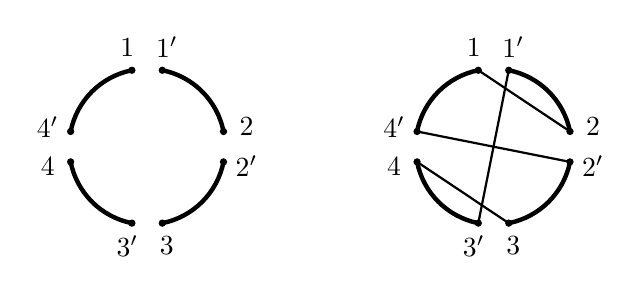
\begin{tikzpicture}[scale=0.55]
		\draw[ultra thick] (-0.351,1.765) arc (101.25:168.75:1.8);
		\filldraw (1.765,0.351) circle (2pt);
		\filldraw (1.765,-0.351) circle (2pt);
		%\draw [dotted,thick] (-0.351,1.765) -- (0.351,1.765);
		\node at (-0.456,2.295) {$1$};
		\node at (0.456,2.295) {$1'$};
		\draw[ultra thick] (1.765,0.351) arc (11.25:78.75:1.8);
		\filldraw (0.351,-1.765) circle (2pt);
		\filldraw (-0.351,-1.765) circle (2pt);
		%\draw [dotted,thick] (1.765,0.351) -- (1.765,-0.351);
		\node at (2.295,0.456) {$2$};
		\node at (2.295,-0.456) {$2'$};
		\draw[ultra thick] (0.351,-1.765) arc (-78.75:-11.25:1.8);
		\filldraw (-1.765,-0.351) circle (2pt);
		\filldraw (-1.765,0.351) circle (2pt);
		%\draw [dotted,thick] (0.351,-1.765) -- (-0.351,-1.765);
		\node at (0.456,-2.295) {$3$};
		\node at (-0.456,-2.295) {$3'$};
		\draw[ultra thick] (-1.765,-0.351) arc (-168.75:-101.25:1.8);
		\filldraw (-0.351,1.765) circle (2pt);
		\filldraw (0.351,1.765) circle (2pt);
		%\draw [dotted,thick] (-1.765,-0.351) -- (-1.765,0.351);
		\node at (-2.295,-0.456) {$4$};
		\node at (-2.295,0.456) {$4'$};
		
	\tikzset{shift={(-4,0)}}
		
		\draw[ultra thick] (11.648,1.765) arc (101.25:168.75:1.8);
		\filldraw (13.765,0.351) circle (2pt);
		\filldraw (13.765,-0.351) circle (2pt);
		%\draw [dotted,thick] (11.648,1.765) -- (12.351,1.765);
		\node at (11.543,2.295) {$1$};
		\node at (12.456,2.295) {$1'$};
		\draw[ultra thick] (13.765,0.351) arc (11.25:78.75:1.8);
		\filldraw (12.351,-1.765) circle (2pt);
		\filldraw (11.648,-1.765) circle (2pt);
		%\draw [dotted,thick] (13.765,0.351) -- (13.765,-0.351);
		\node at (14.295,0.456) {$2$};
		\node at (14.295,-0.456) {$2'$};
		\draw[ultra thick] (12.351,-1.765) arc (-78.75:-11.25:1.8);
		\filldraw (10.234,-0.351) circle (2pt);
		\filldraw (10.234,0.351) circle (2pt);
		%\draw [dotted,thick] (12.351,-1.765) -- (11.648,-1.765);
		\node at (12.456,-2.295) {$3$};
		\node at (11.543,-2.295) {$3'$};
		\draw[ultra thick] (10.234,-0.351) arc (-168.75:-101.25:1.8);
		\filldraw (11.648,1.765) circle (2pt);
		\filldraw (12.351,1.765) circle (2pt);
		%\draw [dotted,thick] (10.234,-0.351) -- (10.234,0.351);
		\node at (9.704,-0.456) {$4$};
		\node at (9.704,0.456) {$4'$};
		\draw [thick] (11.648,1.765) -- (13.765,0.351);
		\draw [thick] (12.351,1.765) -- (11.648,-1.765);
		\draw [thick] (10.234,-0.351) -- (12.351,-1.765);
		\draw [thick] (13.765,-0.351) -- (10.234,0.351);
		
%		\draw[ultra thick] (-6.465,1.738) arc (105:195:1.8);
%		\filldraw (-4.261,-0.465) circle (2pt);
%		\filldraw (-4.727,-1.272) circle (2pt);
%		%\draw [dotted,thick] (-6.465,1.738) -- (-5.534,1.738);
%		\node at (-6.605,2.26) {$1$};
%		\node at (-5.394,2.26) {$1'$};
%		\draw[ultra thick] (-4.261,-0.465) arc (-15:75:1.8);
%		\filldraw (-7.272,-1.272) circle (2pt);
%		\filldraw (-7.738,-0.465) circle (2pt);
%		%\draw [dotted,thick] (-4.261,-0.465) -- (-4.727,-1.272);
%		\node at (-3.739,-0.605) {$2$};
%		\node at (-4.345,-1.654) {$2'$};
%		\draw[ultra thick] (-7.272,-1.272) arc (-135:-45:1.8);
%		\filldraw (-6.465,1.738) circle (2pt);
%		\filldraw (-5.534,1.738) circle (2pt);
%		%\draw [dotted,thick] (-7.272,-1.272) -- (-7.738,-0.465);
%		\node at (-7.654,-1.654) {$3$};
%		\node at (-8.26,-0.605) {$3'$};
		
%		\draw[ultra thick] (5.534,1.738) arc (105:195:1.8);
%		\filldraw (7.738,-0.465) circle (2pt);
%		\filldraw (7.272,-1.272) circle (2pt);
%		%\draw [dotted,thick] (5.534,1.738) -- (6.465,1.738);
%		\node at (5.394,2.26) {$1$};
%		\node at (6.605,2.26) {$1'$};
%		\draw[ultra thick] (7.738,-0.465) arc (-15:75:1.8);
%		\filldraw (4.727,-1.272) circle (2pt);
%		\filldraw (4.261,-0.465) circle (2pt);
%		%\draw [dotted,thick] (7.738,-0.465) -- (7.272,-1.272);
%		\node at (8.26,-0.605) {$2$};
%		\node at (7.654,-1.654) {$2'$};
%		\draw[ultra thick] (4.727,-1.272) arc (-135:-45:1.8);
%		\filldraw (5.534,1.738) circle (2pt);
%		\filldraw (6.465,1.738) circle (2pt);
%		%\draw [dotted,thick] (4.727,-1.272) -- (4.261,-0.465);
%		\node at (4.345,-1.654) {$3$};
%		\node at (3.739,-0.605) {$3'$};
%		\draw [thick] (5.534,1.738) -- (7.738,-0.465);
%		\draw [thick] (6.465,1.738) -- (4.727,-1.272);
%		\draw [thick] (7.272,-1.272) -- (4.261,-0.465);
	\end{tikzpicture}
\end{center}
\label{fig:draw4}
\caption{Graphical representation of a \opt{4} move}
\end{figure}

Assuming that a full circle represents the tour before the move, 
the points labeled $1,1',\ldots, 4,4'$ are associated to the selection indices
of a generic complete selection $S=(i_1,\ldots, i_4)$ (where a label $l$ represents node $i_l$  
while a label $l'$ represents node $i_l\piu 1$). The  
 arcs $\edg{l}{l'}$ missing from the drawing represent the edges that were removed.

A reinsertion set corresponds to four lines inside the circle which match the points in $\{1,1',\ldots,4,4'\}$ and complete the drawing of a tour (see Fig. \ref{fig:draw4}, right).
Our task will be to identify all such drawings. To simplify the exposition and reduce the number of cases to consider we can exploit the fact that some drawings are symmetric and can be put in one equivalence class.


In general, symmetries of figures in the plane are defined by rotations and reflection along axes of symmetry. In our case there are four rotations and four reflections to consider. 
% Each of them can be represented by a permutation of $\{1,\ldots,3\}$. 
For $j=0,\ldots,3$ let us denote by $\rho_j$ the  rotation of the labels by $j\pi/2$ counterclockwise. Furthermore, we denote by $\psi_x$, $\psi_y$, $\psi_{xy}$ and $\psi_{-xy}$ the reflections along, respectively, the $x$-axis, the $y$-axis, the $(x=y)$-line and the $(x=-y)$-line. The permutations corresponding to these operators are depicted, graphically, in Fig. \ref{fig:symmetries}.


\begin{figure}[h]
\begin{center}
	{\footnotesize
		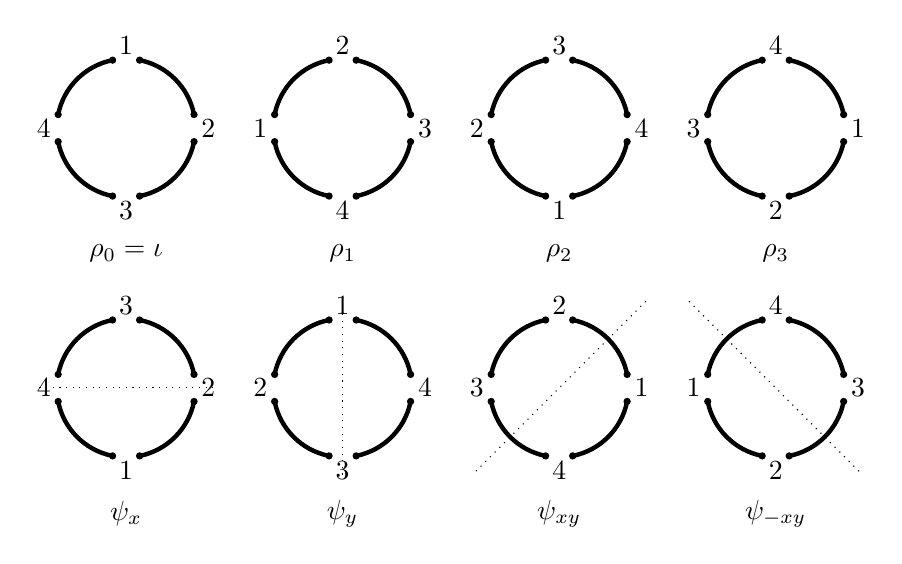
\begin{tikzpicture}[scale=0.55]
			
			\draw[ultra thick] (1.569,0.312) arc (11.25:78.75:1.6);
			\filldraw (0.312,-1.569) circle (2pt);
			\filldraw (-0.312,-1.569) circle (2pt);
			\draw[ultra thick] (0.312,-1.569) arc (-78.75:-11.25:1.6);
			\filldraw (-1.569,-0.312) circle (2pt);
			\filldraw (-1.569,0.312) circle (2pt);
			\draw[ultra thick] (-1.569,-0.312) arc (-168.75:-101.25:1.6);
			\filldraw (-0.312,1.569) circle (2pt);
			\filldraw (0.312,1.569) circle (2pt);
			%\draw [dotted,thick] (-1.569,-0.312) -- (-1.569,0.312);
			\draw[ultra thick] (-0.312,1.569) arc (-258.75:-191.25:1.6);
			\filldraw (1.569,0.312) circle (2pt);
			\filldraw (1.569,-0.312) circle (2pt);
			%\draw [dotted,thick] (-0.312,1.569) -- (0.312,1.569);
			
			
			\node at (0,1.9) {$3$};
			\node at (5,1.9) {$1$};
			\node at (10,1.9) {$2$};
			\node at (15,1.9) {$4$};
			
			\node at (0, -1.9) {$1$}; 
			\node at (5, -1.9) {$3$}; 
			\node at (10, -1.9) {$4$}; 
			\node at (15, -1.9) {$2$}; 
			
			\node at (1.9,0) {2};
			\node at (6.9,0) {4}; 
			\node at (11.9,0) {1}; 
			\node at (16.9,0) {3}; 
			
			\node at (-1.9,0) {4};
			\node at (3.1,0) {2}; 
			\node at (8.1,0) {3}; 
			\node at (13.1,0) {1}; 
			
			
			\node at (0,7.9) {$1$};
			\node at (5,7.9) {$2$};
			\node at (10,7.9) {$3$};
			\node at (15,7.9) {$4$};
			
			\node at (0, 4.1) {$3$}; 
			\node at (5, 4.1) {$4$}; 
			\node at (10, 4.1) {$1$}; 
			\node at (15, 4.1) {$2$}; 
			
			\node at (1.9,6) {2};
			\node at (6.9,6) {3}; 
			\node at (11.9,6) {4}; 
			\node at (16.9,6) {1}; 
			
			\node at (-1.9,6) {4};
			\node at (3.1,6) {1}; 
			\node at (8.1,6) {2}; 
			\node at (13.1,6) {3}; 
			
			\node at (0, 3.1) {$\rho_0=\iota$}; 
			\node at (5, 3.1) {$\rho_1$}; 
			\node at (10, 3.1) {$\rho_2$};      
			\node at (15, 3.1) {$\rho_3$}; 
			\node at (0, -2.9) {$\psi_x$}; 
			\node at (5, -2.9) {$\psi_y$}; 
			\node at (10, -2.9) {$\psi_{xy}$};      
			\node at (15, -2.9) {$\psi_{-xy}$}; 
			
			\draw[ultra thick] (6.569,0.312) arc (11.25:78.75:1.6);
			\filldraw (5.312,-1.569) circle (2pt);
			\filldraw (4.687,-1.569) circle (2pt);
			%\draw [dotted,thick] (6.569,0.312) -- (6.569,-0.312);
			\draw[ultra thick] (5.312,-1.569) arc (-78.75:-11.25:1.6);
			\filldraw (3.43,-0.312) circle (2pt);
			\filldraw (3.43,0.312) circle (2pt);
			%\draw [dotted,thick] (5.312,-1.569) -- (4.687,-1.569);
			\draw[ultra thick] (3.43,-0.312) arc (-168.75:-101.25:1.6);
			\filldraw (4.687,1.569) circle (2pt);
			\filldraw (5.312,1.569) circle (2pt);
			%\draw [dotted,thick] (3.43,-0.312) -- (3.43,0.312);
			\draw[ultra thick] (4.687,1.569) arc (-258.75:-191.25:1.6);
			\filldraw (6.569,0.312) circle (2pt);
			\filldraw (6.569,-0.312) circle (2pt);
			%\draw [dotted,thick] (4.687,1.569) -- (5.312,1.569);
			
			
			\draw[ultra thick] (11.569,0.312) arc (11.25:78.75:1.6);
			\filldraw (10.312,-1.569) circle (2pt);
			\filldraw (9.687,-1.569) circle (2pt);
			%\draw [dotted,thick] (11.569,0.312) -- (11.569,-0.312);
			\draw[ultra thick] (10.312,-1.569) arc (-78.75:-11.25:1.6);
			\filldraw (8.43,-0.312) circle (2pt);
			\filldraw (8.43,0.312) circle (2pt);
			%\draw [dotted,thick] (10.312,-1.569) -- (9.687,-1.569);
			\draw[ultra thick] (8.43,-0.312) arc (-168.75:-101.25:1.6);
			\filldraw (9.687,1.569) circle (2pt);
			\filldraw (10.312,1.569) circle (2pt);
			%\draw [dotted,thick] (8.43,-0.312) -- (8.43,0.312);
			\draw[ultra thick] (9.687,1.569) arc (-258.75:-191.25:1.6);
			\filldraw (11.569,0.312) circle (2pt);
			\filldraw (11.569,-0.312) circle (2pt);
			%\draw [dotted,thick] (9.687,1.569) -- (10.312,1.569);
			
			\draw[ultra thick] (16.569,0.312) arc (11.25:78.75:1.6);
			\filldraw (15.312,-1.569) circle (2pt);
			\filldraw (14.687,-1.569) circle (2pt);
			\draw[ultra thick] (15.312,-1.569) arc (-78.75:-11.25:1.6);
			\filldraw (13.43,-0.312) circle (2pt);
			\filldraw (13.43,0.312) circle (2pt);
			\draw[ultra thick] (13.43,-0.312) arc (-168.75:-101.25:1.6);
			\filldraw (14.687,1.569) circle (2pt);
			\filldraw (15.312,1.569) circle (2pt);
			%\draw [dotted,thick] (13.43,-0.312) -- (13.43,0.312);
			\draw[ultra thick] (14.687,1.569) arc (-258.75:-191.25:1.6);
			\filldraw (16.569,0.312) circle (2pt);
			\filldraw (16.569,-0.312) circle (2pt);
			%\draw [dotted,thick] (14.687,1.569) -- (15.312,1.569);
			
			
			\draw[ultra thick] (1.569,6.312) arc (11.25:78.75:1.6);
			\filldraw (0.312,4.43) circle (2pt);
			\filldraw (-0.312,4.43) circle (2pt);
			%\draw [dotted,thick] (1.569,6.312) -- (1.569,5.687);
			\draw[ultra thick] (0.312,4.43) arc (-78.75:-11.25:1.6);
			\filldraw (-1.569,5.687) circle (2pt);
			\filldraw (-1.569,6.312) circle (2pt);
			%\draw [dotted,thick] (0.312,4.43) -- (-0.312,4.43);
			\draw[ultra thick] (-1.569,5.687) arc (-168.75:-101.25:1.6);
			\filldraw (-0.312,7.569) circle (2pt);
			\filldraw (0.312,7.569) circle (2pt);
			%\draw [dotted,thick] (-1.569,5.687) -- (-1.569,6.312);
			\draw[ultra thick] (-0.312,7.569) arc (-258.75:-191.25:1.6);
			\filldraw (1.569,6.312) circle (2pt);
			\filldraw (1.569,5.687) circle (2pt);
			%\draw [dotted,thick] (-0.312,7.569) -- (0.312,7.569);
			
			
			\draw[ultra thick] (6.569,6.312) arc (11.25:78.75:1.6);
			\filldraw (5.312,4.43) circle (2pt);
			\filldraw (4.687,4.43) circle (2pt);
			\draw[ultra thick] (5.312,4.43) arc (-78.75:-11.25:1.6);
			\filldraw (3.43,5.687) circle (2pt);
			\filldraw (3.43,6.312) circle (2pt);
			%\draw [dotted,thick] (5.312,4.43) -- (4.687,4.43);
			\draw[ultra thick] (3.43,5.687) arc (-168.75:-101.25:1.6);
			\filldraw (4.687,7.569) circle (2pt);
			\filldraw (5.312,7.569) circle (2pt);
			%\draw [dotted,thick] (3.43,5.687) -- (3.43,6.312);
			\draw[ultra thick] (4.687,7.569) arc (-258.75:-191.25:1.6);
			\filldraw (6.569,6.312) circle (2pt);
			\filldraw (6.569,5.687) circle (2pt);
			%\draw [dotted,thick] (4.687,7.569) -- (5.312,7.569);
			
			
			
			\draw[ultra thick] (11.569,6.312) arc (11.25:78.75:1.6);
			\filldraw (10.312,4.43) circle (2pt);
			\filldraw (9.687,4.43) circle (2pt);
			%\draw [dotted,thick] (11.569,6.312) -- (11.569,5.687);
			\draw[ultra thick] (10.312,4.43) arc (-78.75:-11.25:1.6);
			\filldraw (8.43,5.687) circle (2pt);
			\filldraw (8.43,6.312) circle (2pt);
			%\draw [dotted,thick] (10.312,4.43) -- (9.687,4.43);
			\draw[ultra thick] (8.43,5.687) arc (-168.75:-101.25:1.6);
			\filldraw (9.687,7.569) circle (2pt);
			\filldraw (10.312,7.569) circle (2pt);
			\draw[ultra thick] (9.687,7.569) arc (-258.75:-191.25:1.6);
			\filldraw (11.569,6.312) circle (2pt);
			\filldraw (11.569,5.687) circle (2pt);
			
			
			\draw[ultra thick] (16.569,6.312) arc (11.25:78.75:1.6);
			\filldraw (15.312,4.43) circle (2pt);
			\filldraw (14.687,4.43) circle (2pt);
			\draw[ultra thick] (15.312,4.43) arc (-78.75:-11.25:1.6);
			\filldraw (13.43,5.687) circle (2pt);
			\filldraw (13.43,6.312) circle (2pt);
			\draw[ultra thick] (13.43,5.687) arc (-168.75:-101.25:1.6);
			\filldraw (14.687,7.569) circle (2pt);
			\filldraw (15.312,7.569) circle (2pt);
			\draw[ultra thick] (14.687,7.569) arc (-258.75:-191.25:1.6);
			\filldraw (16.569,6.312) circle (2pt);
			\filldraw (16.569,5.687) circle (2pt);
			
			% 	    \draw [dotted] (0,4) -- (0,8);
			% 	    \draw [dotted] (-2,6) -- (2,6);
			% 	    \draw [dotted] (-2,8) -- (2,4);
			% 	    \draw [dotted] (2,8) -- (-2,4);
			
			
			\draw [dotted] (5,-2) -- (5,2);
			\draw [dotted] (-2,0) -- (2,0);
			%	    \draw [dotted] (-2,8) -- (2,4);
			%	    \draw [dotted] (2,8) -- (-2,4);
			\draw [dotted] (13,2) -- (17,-2);
			\draw [dotted] (12,2) -- (8,-2);
			
		\end{tikzpicture}
	}
\caption{The set of all symmetry operators applied to a tour}
	\label{fig:symmetries}
\end{center}
\end{figure}

The set ${\cal G}=\{\rho_0,\rho_1,\rho_2,\rho_3,\psi_{x} 
,\psi_{y},\psi_{xy},\psi_{-xy}\}$ is a group, of order four, under the operation of function composition. In algebra it is known as the {\em octic} group. The identity is $\rho_0$. Let $\rho=\rho_1$ and $\psi=\psi_x$. Then we have $\rho_j=\rho^j$ and $\psi_y = \psi \rho^2$, 
$\psi_{xy} = \psi \rho^3$, 
$\psi_{-xy} = \psi \rho$, so that 
%$\rho$ and $\psi$ are sufficient to generate ${\cal G}$ and
${\cal G}=\{\rho^j,\psi\rho^j, j=0,\ldots,3\}$.
To define equivalent (i.e., symmetric) reinsertion sets,
we  need to apply some results from the algebraic theory of group actions. We define a group action of ${\cal G}$ on $\reinsset(S)$ by specifying, for each $\varphi\in {\cal G}$ and $I\in \reinsset(S)$ a set $\varphi I\in\reinsset(S)$. For each $\varphi\in {\cal G}$, this association must be  a bijection of  $\reinsset(S)$ into itself.


Let us then define new labels for each node $x$, $x'$ with $x=1,\ldots,4$, under the action of $\varphi$ as
\beq
\begin{cases}
	L_{\varphi}(x)=\varphi(x)\quad\ L_{\varphi}(x') =\varphi(x)' \qquad \textrm{ if } \varphi=\rho^j \textrm{ for some } j\\
	L_{\varphi}(x)=\varphi(x)'\quad L_{\varphi}(x') =\varphi(x)\, \qquad \textrm{ otherwise}\\
\end{cases}
\label{def:L}
\eeq
Then a reinsertion set $I$ is mapped by $\varphi$ into the reinsertion set
\[
\varphi I :=\big\{\edg{L_{\varphi}(x)}{L_{\varphi}(y)} : \edg{x}{y}\in I\big\}
\]

Two reinsertion sets $I$ and $I'$ are said to be symmetric if there exists $\varphi\in{\cal G}$ such that $I'=\varphi I$. This relation is in fact an equivalence. The equivalence class $\orbit{I}=\{\varphi I:  \varphi\in {\cal G}\}$ is called the {\em orbit} of $I$. The orbits partition the set $\reinsset(S)$. It is a known result from algebra that in a group action the size of an orbit must divide the size of the group. Therefore, in \opt{4} each orbit  must have 1, 2, 4 or 8 elements.

\begin{figure}[t]
\begin{center}
	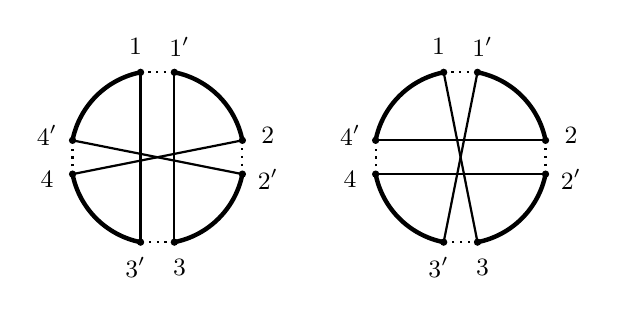
\begin{tikzpicture}[scale=0.55]
		\draw[ultra thick] (-0.39,1.961) arc (101.25:168.75:2);
		\filldraw (1.961,0.39) circle (2pt);
		\filldraw (1.961,-0.39) circle (2pt);
		\draw [dotted,thick] (-0.39,1.961) -- (0.39,1.961);
		\node at (-0.507,2.55) {{\small $1$}};
		\node at (0.507,2.55) {\small $1'$};
		\draw[ultra thick] (1.961,0.39) arc (11.25:78.75:2);
		\filldraw (0.39,-1.961) circle (2pt);
		\filldraw (-0.39,-1.961) circle (2pt);
		\draw [dotted,thick] (1.961,0.39) -- (1.961,-0.39);
		\node at (2.55,0.507) {\small $2$};
		\node at (2.55,-0.507) {\small $2'$};
		\draw[ultra thick] (0.39,-1.961) arc (-78.75:-11.25:2);
		\filldraw (-1.961,-0.39) circle (2pt);
		\filldraw (-1.961,0.39) circle (2pt);
		\draw [dotted,thick] (0.39,-1.961) -- (-0.39,-1.961);
		\node at (0.507,-2.55) {\small $3$};
		\node at (-0.507,-2.55) {\small $3'$};
		\draw[ultra thick] (-1.961,-0.39) arc (-168.75:-101.25:2);
		\filldraw (-0.39,1.961) circle (2pt);
		\filldraw (0.39,1.961) circle (2pt);
		\draw [dotted,thick] (-1.961,-0.39) -- (-1.961,0.39);
		\node at (-2.55,-0.507) {\small $4$};
		\node at (-2.55,0.507) {\small $4'$};
		\draw [thick] (-0.39,1.961) -- (-0.39,-1.961);
		\draw [thick] (-1.961,-0.39) -- (1.961,0.39);
		\draw [thick] (0.39,1.961) -- (0.39,-1.961);
		\draw [thick] (1.961,-0.39) -- (-1.961,0.39);
		
		\draw[ultra thick] (6.609,1.961) arc (101.25:168.75:2);
		\filldraw (8.961,0.39) circle (2pt);
		\filldraw (8.961,-0.39) circle (2pt);
		\draw [dotted,thick] (6.609,1.961) -- (7.39,1.961);
		\node at (6.492,2.55) {\small $1$};
		\node at (7.507,2.55) {\small $1'$};
		\draw[ultra thick] (8.961,0.39) arc (11.25:78.75:2);
		\filldraw (7.39,-1.961) circle (2pt);
		\filldraw (6.609,-1.961) circle (2pt);
		\draw [dotted,thick] (8.961,0.39) -- (8.961,-0.39);
		\node at (9.55,0.507) {\small $2$};
		\node at (9.55,-0.507) {\small $2'$};
		\draw[ultra thick] (7.39,-1.961) arc (-78.75:-11.25:2);
		\filldraw (5.038,-0.39) circle (2pt);
		\filldraw (5.038,0.39) circle (2pt);
		\draw [dotted,thick] (7.39,-1.961) -- (6.609,-1.961);
		\node at (7.507,-2.55) {\small $3$};
		\node at (6.492,-2.55) {\small $3'$};
		\draw[ultra thick] (5.038,-0.39) arc (-168.75:-101.25:2);
		\filldraw (6.609,1.961) circle (2pt);
		\filldraw (7.39,1.961) circle (2pt);
		\draw [dotted,thick] (5.038,-0.39) -- (5.038,0.39);
		\node at (4.449,-0.507) {\small $4$};
		\node at (4.449,0.507) {\small $4'$};
		\draw [thick] (6.609,1.961) -- (7.39,-1.961);
		\draw [thick] (8.961,-0.39) -- (5.038,-0.39);
		\draw [thick] (6.609,-1.961) -- (7.39,1.961);
		\draw [thick] (8.961,0.39) -- (5.038,0.39);
		
	\end{tikzpicture}
\end{center}
\caption{A reinsertion set before and after a rotation}
\label{fig:rot}
\end{figure}


Consider, for example, the reinsertion set $\{\edg{i_1}{i_3\piu 1}, \edg{i_1\piu 1}{i_3},\edg{i_2}{i_4}, \edg{i_2\piu 1}{i_4\piu 1}\}$ which, in our notation, is
\[
I=\{\edg{1}{3'}, \edg{1'}{3},\edg{2}{4}, \edg{2'}{4'}\}
\]
and is depicted in Fig. \ref{fig:rot}(left). 
If we apply a rotation $\rho$ we obtain the set
\begin{align*}
\rho I &=\{\edg{\rho({1})}{\rho({3})'}, \edg{\rho({1})'}{\rho({3})},\edg{\rho({2})}{\rho({4})}, \edg{\rho({2})'}{\rho({4})'}\}\\
 & =\{\edg{2}{4'}, \edg{2'}{4},\edg{3}{1}, \edg{3'}{1'}\}
\end{align*}

which is depicted in Fig. \ref{fig:rot}(right) and corresponds to the actual edges 
$\{\edg{i_1}{i_3}, \edg{i_1\piu 1}{i_3\piu 1},\edg{i_2}{i_4\piu 1}, \edg{i_2\piu 1}{i_4}\}$. If we apply the rotation $\rho$ again we obtain 
\begin{align*}
\rho^2 I & = \{\edg{\rho({2})}{\rho(4)'}, \edg{\rho(2)'}{\rho({4})},\edg{\rho({3})}{\rho({1})}, \edg{\rho({3})'}{\rho({1})'}\}\\
& =\{\edg{3}{1'}, \edg{3'}{1},\edg{4}{2}, \edg{4'}{2'}\}\\
& =I
\end{align*}
Similarly,
\begin{align*}
\psi I &=\{\edg{\psi(1)'}{\psi({3})}, \edg{\psi(1)}{\psi({3})'},\edg{\psi({2})'}{\psi({4})'}, \edg{\psi({2})}{\psi({4})}\}\\
 & =\{\edg{3'}{1}, \edg{3}{1'},\edg{2}{4}, \edg{2'}{4'}\}\\
 & =I
\end{align*}

Therefore $\orbit{I}=\{I,\rho I\}$ and the orbit has size 2.



In order  to enumerate all the reinsertion sets so as to compute their orbits and partition them into a small number of cases, we introduce a handy notation called {\em reinsertion schemes}. Reinsertion schemes will be in 1-to-1 correspondence with reinsertion sets.



\subsection{Reinsertion schemes}
\label{sec:comb}

Let $S$ be a complete \opt{4} selection.
When the edges $R(S)$ are removed from a tour, the tour
gets broken into four segments  which we label by $\{1,\ldots,4\}$. For $l=1,\ldots,4$, the  segment labeled $l$ is the path that has  $i_l$ as its last vertex. In particular, the segments are $(i_4\piu 1,\ldots, i_1)$, $(i_1\piu 1,\ldots,  i_2)$,
$(i_2\piu 1,\ldots, i_3)$ and $(i_3\piu 1,\ldots, i_4)$.
Since the selection is pure, each segment contains at least one edge. A reinsertion set 
patches back these segments into a new tour. If we adopt the convention to start always a tour with segment 1 traversed clockwise, 
the reinsertion set: (i) determines a new ordering in which the segments are visited along the tour and (ii) may cause some segments to be traversed counterclockwise.
In order to represent this fact, instead of listing the edges of a reinsertion set we can use an alternative notation called a {\em reinsertion scheme}. A reinsertion scheme is a signed permutation of $\{2,3,4\}$. The permutation specifies the order in which the segments $2,3,4$ are visited after the move. The signing $-s$ tells that segment $s$ is traversed counterclockwise, while $+s$ tells that it is traversed clockwise. 
For example, the reinsertion set depicted in Fig. \ref{fig:rot}(left) is also represented by the reinsertion scheme
$\Reinss{+4}{-2}{-3}$ since  from the end of segment 1  we jump to the beginning of segment 4 and traverse the segment forward. We then move to the last element of  segment 2 and proceed backward to its first element. We then jump to the end of segment 3 and proceed backward to its beginning. Finally, we close the cycle by going back to the first element of segment 1. 

\iffalse
\begin{figure}[t]
	\begin{center}
		{\small
			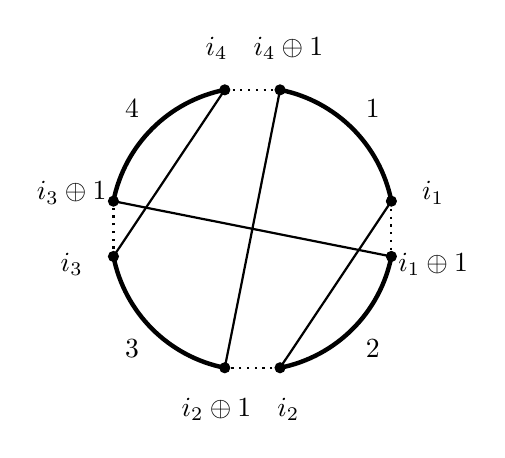
\begin{tikzpicture}[scale=0.9]
				\draw[ultra thick] (1.961,0.39) arc (11.25:78.75:2);
				\filldraw (0.39,-1.961) circle (2pt);
				\filldraw (-0.39,-1.961) circle (2pt);
				\draw [dotted,thick] (1.961,0.39) -- (1.961,-0.39);
				\node at (2.55,0.507) {$i_1$};
				\node at (2.55,-0.507) {$i_1\piu 1$};
				\node at (1.697,1.697) {$1$};
				\draw[ultra thick] (0.39,-1.961) arc (-78.75:-11.25:2);
				\filldraw (-1.961,-0.39) circle (2pt);
				\filldraw (-1.961,0.39) circle (2pt);
				\draw [dotted,thick] (0.39,-1.961) -- (-0.39,-1.961);
				\node at (0.507,-2.55) {$i_2$};
				\node at (-0.507,-2.55) {$i_2\piu 1$};
				\node at (1.697,-1.697) {$2$};
				\draw[ultra thick] (-1.961,-0.39) arc (-168.75:-101.25:2);
				\filldraw (-0.39,1.961) circle (2pt);
				\filldraw (0.39,1.961) circle (2pt);
				\draw [dotted,thick] (-1.961,-0.39) -- (-1.961,0.39);
				\node at (-2.55,-0.507) {$i_3$};
				\node at (-2.55,0.507) {$i_3\piu 1$};
				\node at (-1.697,-1.697) {$3$};
				\draw[ultra thick] (-0.39,1.961) arc (-258.75:-191.25:2);
				\filldraw (1.961,0.39) circle (2pt);
				\filldraw (1.961,-0.39) circle (2pt);
				\draw [dotted,thick] (-0.39,1.961) -- (0.39,1.961);
				\node at (-0.507,2.55) {$i_4$};
				\node at (0.507,2.55) {$i_4\piu 1$};
				\node at (-1.697,1.697) {$4$};
				\draw [thick] (1.961,0.39) -- (0.39,-1.961);
				\draw [thick] (1.961,-0.39) -- (-1.961,0.39);
				\draw [thick] (-0.39,1.961) -- (-1.961,-0.39);
				\draw [thick] (-0.39,-1.961) -- (0.39,1.961);
			\end{tikzpicture}
		}
		\caption{The reinsertion scheme $\Reinss{-2}{+4}{-3}$}
		\label{fig:reins4}
	\end{center}
\end{figure}
\fi


Clearly, there is a bijection between reinsertion schemes and reinsertion sets. If $r$ is a reinsertion scheme,  we denote by $I(r)$ 
the corresponding reinsertion set, while if $I$ is a reinsertion set, we denote by $r(I)$ the corresponding reinsertion scheme. We can then readily extend the idea of orbits and group actions to reinsertion schemes. Namely, we will consider the orbit of a reinsertion scheme to be the set of all reinsertion schemes whose corresponding reinsertion sets are symmetric. Let $I$ be a reinsertion set, and $r=r(I)$. Then  we extend the action of ${\cal G}$ to reinsertion schemes by defining, for each $\varphi\in{\cal G}$, the scheme $\varphi r$ to be
$r(\varphi I)$. For example, by looking at Fig. \ref{fig:rot}(b) we have that $\rho \Reinss{-2}{+4}{-3} = \Reinss{-3}{-4}{+2}$.
Because of the equivalence between reinsertion sets and reinsertion schemes, in the following we will be using either of them, at our convenience, for the sake of simplicity. 

There are potentially $2^{3}\times 3!$ reinsertion schemes for \opt{4}, but for many of these the corresponding reinsertion sets are degenerate. A scheme for a pure reinsertion  must not  start with $+2$, nor end with ``$+4$'', nor contain consecutive elements ``$+t,+(t+1)$'' or ``$-t,-(t-1)$'' for any $t$ in $1,\ldots,4$.

\begin{proposition}
	There are 25 pure reinsertion schemes for \opt{4}.
\end{proposition}

\begin{proof} 
The pure schemes, classified by a permutation $\pi$ of $\{2,3,4\}$ first and then by the signing, are the following:
	\begin{enumerate}
		\item [-] $\pi=(2,3,4)$: Signing $+2$ is forbidden, and also $+4$ is forbidden. This leaves only two possibilities
		\begin{enumerate}
			\item [] $\rq{1}=\Reinss{-2}{-3}{-4}$\qquad \qquad $\rq{2}=\Reinss{-2}{+3}{-4}$
		\end{enumerate}
		\item [-] $\pi=(2,4,3)$: Signing $+2$ is forbidden. Also the sequence $-4,-3$ is forbidden. This leaves three possibilities
		\begin{enumerate}
			\item [] $\rq{3}=\Reinss{-2}{-4}{+3}$ \qquad \qquad
			$\rq{4} = \Reinss{-2}{+4}{-3}$ \qquad \qquad
			$\rq{5} = \Reinss{-2}{+4}{+3}$
		\end{enumerate}
		%(See figure \ref{fig:4optab} for reinsertion schemes starting with $a,b$.)
		%\begin{figure}[t]
		%\begin{center}
		%\adjustbox{trim={0\width} {0.3\height} {0\width} {0\height},clip}%
		%{\includegraphics[width=14cm]{4opt_ab.pdf}}
		%\end{center}
		%\caption{Reinsertion schemes starting with $a,b$}
		%\label{fig:4optab}
		%\end{figure}
		
		\item [-] $\pi=(3,2,4)$: Signing $+4$ is forbidden. Also the sequence $-3,-2$ is forbidden. This leaves three possibilities
		\begin{enumerate}
			\item [] $\rq{6} = \Reinss{-3}{+2}{-4}$ \qquad \qquad
			$\rq{7} = \Reinss{+3}{-2}{-4}$ \qquad \qquad
			$\rq{8} = \Reinss{+3}{+2}{-4}$
		\end{enumerate}
		
		\item [-] $\pi=(3,4,2)$: The sequence $+3,+4$ is forbidden. This leaves six possibilities
		\begin{enumerate}
			\item[] $\rq{9} = \Reinss{-3}{-4}{-2}$ \qquad \qquad
			$\rq{10} = \Reinss{-3}{-4}{+2}$ \qquad \qquad
			$\rq{11} = \Reinss{-3}{+4}{-2}$ 
			\item [] $\rq{12} = \Reinss{-3}{+4}{+2}$ \qquad \quad\
			$\rq{13} = \Reinss{+3}{-4}{-2}$ \qquad \qquad
			$\rq{14} = \Reinss{+3}{-4}{+2}$
		\end{enumerate}
		%	(See figure \ref{fig:4optac} for reinsertion schemes starting with $a,c$.)
		%	
		%	\begin{figure}[h]
		%	\begin{center}
		%	\adjustbox{trim={0\width} {0\height} {0\width} {0\height},clip}%
		%	{\includegraphics[width=14cm]{4opt_ac.pdf}}
		%	\end{center}
		%	\caption{Reinsertion schemes starting with $a,c$}
		%		\label{fig:4optac}
		%	\end{figure}
		%	
		\item [-] $\pi=(4,2,3)$: The sequence $+2,+3$ is forbidden. This leaves six possibilities
		\begin{enumerate}
			\item[] $\rq{15} = \Reinss{-4}{-2}{-3}$ \qquad \qquad
			$\rq{16} = \Reinss{+4}{-2}{-3}$ \qquad \qquad
			$\rq{17} = \Reinss{-4}{-2}{+3}$
			\item[] $\rq{18} = \Reinss{+4}{-2}{+3}$ \qquad \qquad
			$\rq{19} = \Reinss{-4}{+2}{-3}$\qquad \qquad
			$\rq{20} = \Reinss{+4}{+2}{-3}$
		\end{enumerate}
		%		(See figure \ref{fig:4optadb} for reinsertion schemes starting with $a,d,b$.)
		%		
		%	\begin{figure}[h]
		%	\begin{center}
		%	\adjustbox{trim={0\width} {0.35\height} {0\width} {0\height},clip}%
		%	{\includegraphics[width=14cm]{4opt_adb.pdf}}
		%	\end{center}
		%	\caption{Reinsertion schemes starting with $a,d,b$}
		%	\label{fig:4optadb}
		%	\end{figure}
		%	
		\item [-] $\pi=(4,3,2)$ : The sequence $-4,-3$ is forbidden as well as the sequence $-3,-2$. This leaves five possibilities
		\begin{enumerate}
			\item[] $\rq{21} = \Reinss{-4}{+3}{-2}$ \qquad \qquad
			$\rq{22} = \Reinss{-4}{+3}{+2}$ \qquad \qquad
			$\rq{23} = \Reinss{+4}{-3}{+2}$
			\item[] $\rq{24} = \Reinss{+4}{+3}{-2}$ \qquad \qquad
			$\rq{25} = \Reinss{+4}{+3}{+2}$
		\end{enumerate}
		%	(See figure \ref{fig:4optadc} for reinsertion schemes starting with $a,d,c$.)
		%	
		%	\begin{figure}[h]
		%	\begin{center}
		%	\adjustbox{trim={0\width} {0.3\height} {0\width} {0\height},clip}%
		%	{\includegraphics[width=14cm]{4opt_adc.pdf}}
		%	\end{center}
		%	\caption{Reinsertion schemes starting with $a,d,c$}
		%	\label{fig:4optadc}
		%	\end{figure}
		
	\end{enumerate}
\end{proof}
We can now proceed and compute the orbits for the pure reinsertion schemes.

\begin{proposition}
	The pure reinsertion schemes for \opt{4} are partitioned in  7 orbits ${\cal O}_1,\ldots,{\cal O}_7$.
\end{proposition}
\begin{proof}
	We have 
	\begin{enumerate}
		\item [-] ${\cal O}_1=\orbit{\rq{1}}=\{\rq{1},\rq{24},\rq{23},\rq{22}\} = 
		\{\rq{1}, \rho\rq{1}, \rho^2\rq{1}, \rho^3\rq{1}\}$.
		\item [-] ${\cal O}_2=\orbit{\rq{2}}=\{\rq{2},\rq{21}\} = \{\rq{2},\rho\rq{2}\}$.
		\item [-] ${\cal O}_3=\orbit{\rq{3}}=\{\rq{3},\rq{7},\rq{13},\rq{17}\} = \{\rq{3},\rho\rq{3},\rho^2\rq{3}, \rho^3\rq{3}\}$.
		\item [-] ${\cal O}_4=\orbit{\rq{4}}=\{\rq{4},\rq{19},\rq{11},\rq{6}\} = \{\rq{4},\rho\rq{4},\psi\rq{4}, \psi\rho\rq{4}\}$.
		\item [-] ${\cal O}_5=\orbit{\rq{5}}=\{\rq{5},\rq{20},\rq{14},\rq{15},\rq{12},\rq{18},\rq{9},\rq{8}\} = \{\rq{5},\rho\rq{5},\rho^2\rq{5},\rho^3\rq{5},\psi\rq{5}, \psi\rho\rq{5},\psi\rho^2\rq{5}, \psi\rho^3\rq{5}\}$.
		\item [-] ${\cal O}_6=\orbit{\rq{10}}=\{\rq{10},\rq{16}\}=\{\rq{10},\rho\rq{10}\}$.
		\item [-] ${\cal O}_7=\orbit{\rq{25}}=\{\rq{25}\}$.
	\end{enumerate}
\end{proof}


\begin{figure}[tb]
	\begin{center}
		{\footnotesize
			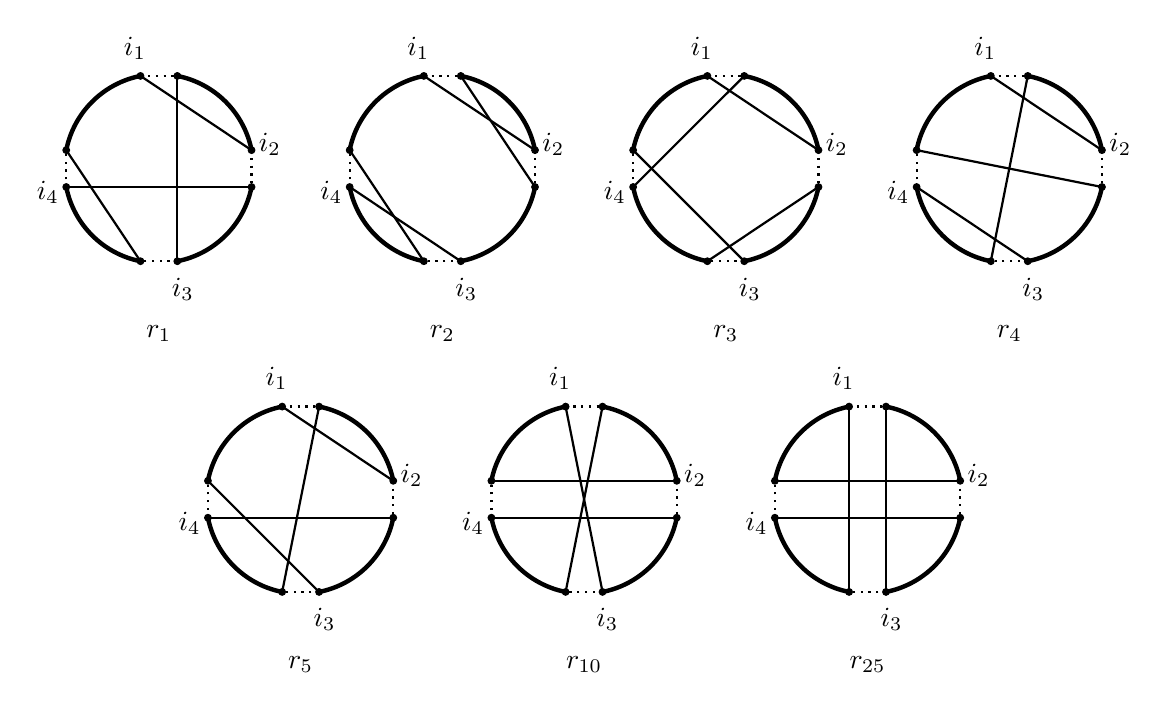
\begin{tikzpicture}[scale=0.6]
				\draw[ultra thick] (-0.39,1.961) arc (101.25:168.75:2);
				\filldraw (1.961,0.39) circle (2pt);
				\filldraw (1.961,-0.39) circle (2pt);
				\draw [dotted,thick] (-0.39,1.961) -- (0.39,1.961);
				\node at (-0.507,2.55) {$i_1$};
%				\node at (0.507,2.55) {$i_1\piu 1$};
				\draw[ultra thick] (1.961,0.39) arc (11.25:78.75:2);
				\filldraw (0.39,-1.961) circle (2pt);
				\filldraw (-0.39,-1.961) circle (2pt);
				\draw [dotted,thick] (1.961,0.39) -- (1.961,-0.39);
				\node at (2.35,0.507) {$i_2$};
%				\node at (2.55,-0.507) {$i_2\piu 1$};
				\draw[ultra thick] (0.39,-1.961) arc (-78.75:-11.25:2);
				\filldraw (-1.961,-0.39) circle (2pt);
				\filldraw (-1.961,0.39) circle (2pt);
				\draw [dotted,thick] (0.39,-1.961) -- (-0.39,-1.961);
				\node at (0.507,-2.55) {$i_3$};
%				\node at (-0.507,-2.55) {$i_3\piu 1$};
				\draw[ultra thick] (-1.961,-0.39) arc (-168.75:-101.25:2);
				\filldraw (-0.39,1.961) circle (2pt);
				\filldraw (0.39,1.961) circle (2pt);
				\draw [dotted,thick] (-1.961,-0.39) -- (-1.961,0.39);
				\node at (-2.35,-0.507) {$i_4$};
%				\node at (-2.55,0.507) {$i_4\piu 1$};
				\draw [thick] (-0.39,1.961) -- (1.961,0.39);
				\draw [thick] (0.39,1.961) -- (0.39,-1.961);
				\draw [thick] (1.961,-0.39) -- (-1.961,-0.39);
				\draw [thick] (-0.39,-1.961) -- (-1.961,0.39);
				
				
				\draw[ultra thick] (5.609,1.961) arc (101.25:168.75:2);
				\filldraw (7.961,0.39) circle (2pt);
				\filldraw (7.961,-0.39) circle (2pt);
				\draw [dotted,thick] (5.609,1.961) -- (6.39,1.961);
				\node at (5.492,2.55) {$i_1$};
%				\node at (6.507,2.55) {$i_1\piu 1$};
				\draw[ultra thick] (7.961,0.39) arc (11.25:78.75:2);
				\filldraw (6.39,-1.961) circle (2pt);
				\filldraw (5.609,-1.961) circle (2pt);
				\draw [dotted,thick] (7.961,0.39) -- (7.961,-0.39);
				\node at (8.35,0.507) {$i_2$};
%				\node at (8.55,-0.507) {$i_2\piu 1$};
				\draw[ultra thick] (6.39,-1.961) arc (-78.75:-11.25:2);
				\filldraw (4.038,-0.39) circle (2pt);
				\filldraw (4.038,0.39) circle (2pt);
				\draw [dotted,thick] (6.39,-1.961) -- (5.609,-1.961);
				\node at (6.507,-2.55) {$i_3$};
%				\node at (5.492,-2.55) {$i_3\piu 1$};
				\draw[ultra thick] (4.038,-0.39) arc (-168.75:-101.25:2);
				\filldraw (5.609,1.961) circle (2pt);
				\filldraw (6.39,1.961) circle (2pt);
				\draw [dotted,thick] (4.038,-0.39) -- (4.038,0.39);
				\node at (3.649,-0.507) {$i_4$};
%				\node at (3.449,0.507) {$i_4\piu 1$};
				\draw [thick] (5.609,1.961) -- (7.961,0.39);
				\draw [thick] (6.39,1.961) -- (7.961,-0.39);
				\draw [thick] (6.39,-1.961) -- (4.038,-0.39);
				\draw [thick] (5.609,-1.961) -- (4.038,0.39);
				
				\draw[ultra thick] (11.609,1.961) arc (101.25:168.75:2);
				\filldraw (13.961,0.39) circle (2pt);
				\filldraw (13.961,-0.39) circle (2pt);
				\draw [dotted,thick] (11.609,1.961) -- (12.39,1.961);
				\node at (11.492,2.55) {$i_1$};
%				\node at (12.507,2.55) {$i_1\piu 1$};
				\draw[ultra thick] (13.961,0.39) arc (11.25:78.75:2);
				\filldraw (12.39,-1.961) circle (2pt);
				\filldraw (11.609,-1.961) circle (2pt);
				\draw [dotted,thick] (13.961,0.39) -- (13.961,-0.39);
				\node at (14.35,0.507) {$i_2$};
%				\node at (14.55,-0.507) {$i_2\piu 1$};
				\draw[ultra thick] (12.39,-1.961) arc (-78.75:-11.25:2);
				\filldraw (10.038,-0.39) circle (2pt);
				\filldraw (10.038,0.39) circle (2pt);
				\draw [dotted,thick] (12.39,-1.961) -- (11.609,-1.961);
				\node at (12.507,-2.55) {$i_3$};
%				\node at (11.492,-2.55) {$i_3\piu 1$};
				\draw[ultra thick] (10.038,-0.39) arc (-168.75:-101.25:2);
				\filldraw (11.609,1.961) circle (2pt);
				\filldraw (12.39,1.961) circle (2pt);
				\draw [dotted,thick] (10.038,-0.39) -- (10.038,0.39);
				\node at (9.649,-0.507) {$i_4$};
%				\node at (9.449,0.507) {$i_4\piu 1$};
				\draw [thick] (11.609,1.961) -- (13.961,0.39);
				\draw [thick] (12.39,1.961) -- (10.038,-0.39);
				\draw [thick] (11.609,-1.961) -- (13.961,-0.39);
				\draw [thick] (12.39,-1.961) -- (10.038,0.39);
				
				
				\draw[ultra thick] (17.609,1.961) arc (101.25:168.75:2);
				\filldraw (19.961,0.39) circle (2pt);
				\filldraw (19.961,-0.39) circle (2pt);
				\draw [dotted,thick] (17.609,1.961) -- (18.39,1.961);
				\node at (17.492,2.55) {$i_1$};
%				\node at (18.507,2.55) {$i_1\piu 1$};
				\draw[ultra thick] (19.961,0.39) arc (11.25:78.75:2);
				\filldraw (18.39,-1.961) circle (2pt);
				\filldraw (17.609,-1.961) circle (2pt);
				\draw [dotted,thick] (19.961,0.39) -- (19.961,-0.39);
				\node at (20.35,0.507) {$i_2$};
%				\node at (20.55,-0.507) {$i_2\piu 1$};
				\draw[ultra thick] (18.39,-1.961) arc (-78.75:-11.25:2);
				\filldraw (16.038,-0.39) circle (2pt);
				\filldraw (16.038,0.39) circle (2pt);
				\draw [dotted,thick] (18.39,-1.961) -- (17.609,-1.961);
				\node at (18.507,-2.55) {$i_3$};
%				\node at (17.492,-2.55) {$i_3\piu 1$};
				\draw[ultra thick] (16.038,-0.39) arc (-168.75:-101.25:2);
				\filldraw (17.609,1.961) circle (2pt);
				\filldraw (18.39,1.961) circle (2pt);
				\draw [dotted,thick] (16.038,-0.39) -- (16.038,0.39);
				\node at (15.649,-0.507) {$i_4$};
%				\node at (15.449,0.507) {$i_4\piu 1$};
				\draw [thick] (17.609,1.961) -- (19.961,0.39);
				\draw [thick] (18.39,1.961) -- (17.609,-1.961);
				\draw [thick] (16.038,-0.39) -- (18.39,-1.961);
				\draw [thick] (19.961,-0.39) -- (16.038,0.39);
				
				\draw[ultra thick] (2.609,-5.038) arc (101.25:168.75:2);
				\filldraw (4.961,-6.609) circle (2pt);
				\filldraw (4.961,-7.39) circle (2pt);
				\draw [dotted,thick] (2.609,-5.038) -- (3.39,-5.038);
				\node at (2.492,-4.449) {$i_1$};
%				\node at (3.507,-4.449) {$i_1\piu 1$};
				\draw[ultra thick] (4.961,-6.609) arc (11.25:78.75:2);
				\filldraw (3.39,-8.961) circle (2pt);
				\filldraw (2.609,-8.961) circle (2pt);
				\draw [dotted,thick] (4.961,-6.609) -- (4.961,-7.39);
				\node at (5.35,-6.492) {$i_2$};
%				\node at (5.55,-7.507) {$i_2\piu 1$};
				\draw[ultra thick] (3.39,-8.961) arc (-78.75:-11.25:2);
				\filldraw (1.038,-7.39) circle (2pt);
				\filldraw (1.038,-6.609) circle (2pt);
				\draw [dotted,thick] (3.39,-8.961) -- (2.609,-8.961);
				\node at (3.507,-9.55) {$i_3$};
%				\node at (2.492,-9.55) {$i_3\piu 1$};
				\draw[ultra thick] (1.038,-7.39) arc (-168.75:-101.25:2);
				\filldraw (2.609,-5.038) circle (2pt);
				\filldraw (3.39,-5.038) circle (2pt);
				\draw [dotted,thick] (1.038,-7.39) -- (1.038,-6.609);
				\node at (0.649,-7.507) {$i_4$};
%				\node at (0.449,-6.492) {$i_4\piu 1$};
				\draw [thick] (2.609,-5.038) -- (4.961,-6.609);
				\draw [thick] (3.39,-5.038) -- (2.609,-8.961);
				\draw [thick] (1.038,-7.39) -- (4.961,-7.39);
				\draw [thick] (3.39,-8.961) -- (1.038,-6.609);
				
				
				\draw[ultra thick] (8.609,-5.038) arc (101.25:168.75:2);
				\filldraw (10.961,-6.609) circle (2pt);
				\filldraw (10.961,-7.39) circle (2pt);
				\draw [dotted,thick] (8.609,-5.038) -- (9.39,-5.038);
				\node at (8.492,-4.449) {$i_1$};
%				\node at (9.507,-4.449) {$i_1\piu 1$};
				\draw[ultra thick] (10.961,-6.609) arc (11.25:78.75:2);
				\filldraw (9.39,-8.961) circle (2pt);
				\filldraw (8.609,-8.961) circle (2pt);
				\draw [dotted,thick] (10.961,-6.609) -- (10.961,-7.39);
				\node at (11.35,-6.492) {$i_2$};
%				\node at (11.55,-7.507) {$i_2\piu 1$};
				\draw[ultra thick] (9.39,-8.961) arc (-78.75:-11.25:2);
				\filldraw (7.038,-7.39) circle (2pt);
				\filldraw (7.038,-6.609) circle (2pt);
				\draw [dotted,thick] (9.39,-8.961) -- (8.609,-8.961);
				\node at (9.492,-9.55) {$i_3$};
%				\node at (8.492,-9.55) {$i_3\piu 1$};
				\draw[ultra thick] (7.038,-7.39) arc (-168.75:-101.25:2);
				\filldraw (8.609,-5.038) circle (2pt);
				\filldraw (9.39,-5.038) circle (2pt);
				\draw [dotted,thick] (7.038,-7.39) -- (7.038,-6.609);
				\node at (6.649,-7.507) {$i_4$};
%				\node at (6.449,-6.492) {$i_4\piu 1$};
				\draw [thick] (8.609,-5.038) -- (9.39,-8.961);
				\draw [thick] (10.961,-7.39) -- (7.038,-7.39);
				\draw [thick] (8.609,-8.961) -- (9.39,-5.038);
				\draw [thick] (10.961,-6.609) -- (7.038,-6.609);
				
				\draw[ultra thick] (14.609,-5.038) arc (101.25:168.75:2);
				\filldraw (16.961,-6.609) circle (2pt);
				\filldraw (16.961,-7.39) circle (2pt);
				\draw [dotted,thick] (14.609,-5.038) -- (15.39,-5.038);
				\node at (14.492,-4.449) {$i_1$};
%				\node at (15.507,-4.449) {$i_1\piu 1$};
				\draw[ultra thick] (16.961,-6.609) arc (11.25:78.75:2);
				\filldraw (15.39,-8.961) circle (2pt);
				\filldraw (14.609,-8.961) circle (2pt);
				\draw [dotted,thick] (16.961,-6.609) -- (16.961,-7.39);
				\node at (17.35,-6.492) {$i_2$};
%				\node at (17.55,-7.507) {$i_2\piu 1$};
				\draw[ultra thick] (15.39,-8.961) arc (-78.75:-11.25:2);
				\filldraw (13.038,-7.39) circle (2pt);
				\filldraw (13.038,-6.609) circle (2pt);
				\draw [dotted,thick] (15.39,-8.961) -- (14.609,-8.961);
				\node at (15.507,-9.55) {$i_3$};
%				\node at (14.492,-9.55) {$i_3\piu 1$};
				\draw[ultra thick] (13.038,-7.39) arc (-168.75:-101.25:2);
				\filldraw (14.609,-5.038) circle (2pt);
				\filldraw (15.39,-5.038) circle (2pt);
				\draw [dotted,thick] (13.038,-7.39) -- (13.038,-6.609);
				\node at (12.649,-7.507) {$i_4$};
%				\node at (12.449,-6.492) {$i_4\piu 1$};
				\draw [thick] (14.609,-5.038) -- (14.609,-8.961);
				\draw [thick] (13.038,-7.39) -- (16.961,-7.39);
				\draw [thick] (15.39,-8.961) -- (15.39,-5.038);
				\draw [thick] (16.961,-6.609) -- (13.038,-6.609);
				
				{\normalsize
					\node at (0,-3.5) {$\rq{1}$};
					\node at (6,-3.5) {$\rq{2}$};
					\node at (12,-3.5) {$\rq{3}$};
					\node at (18,-3.5) {$\rq{4}$};
					\node at (3,-10.5) {$\rq{5}$};
					\node at (9,-10.5) {$\rq{10}$};
					\node at (15,-10.5) {$\rq{25}$};
				}
				
			\end{tikzpicture}
		}
		\caption{Orbits of \opt{4}}
		\label{fig:orbits4}
	\end{center}
\end{figure}


We can list all the orbits by specifying just one element, called the {\em representative}, for each of them, since the other elements can be obtained by the action of ${\cal G}$
on the representative. By convention, we have  chosen as the representative the smallest (in lexicographic order) scheme of the orbit.
In Fig. \ref{fig:orbits4} we illustrate the representatives of the 7 orbits. 



\newcommand{\rtrei}{r_1}
%\newcommand{\rtreii}{3O_2}
\newcommand{\rtreii}{r_2}
\newcommand{\rtreiii}{r_3}
\newcommand{\rtreiv}{r_4}



%\footnote{In a sense, each of these moves defines a neighborhood on its own. I.e., a tour could be a local optimum for one of them but not for another, and we could choose to use in our local search only some of them. Obviously there is a trade-off between the type of moves that are used and the time required to optimize the neighborhood. We will address this issue in the section on computational results. Basically, the time needed for all four types of moves is four times larger than when we have only one type. These considerations are not too important for the \opt{3} case in which there are only 4 full reinsertion schemes, but they become important, e.g., in the \opt{4} case in which the full reinsertion schemes are 25. }



 \newcommand{\STOP}{{\tt STOP}}
 \newcommand{\FALSE}{{\tt false}}
 \newcommand{\BEST}{{\tt BESTIMPR}}
%\newcommand{\comment}[1]{\textit{[*#1*]}}
%\newcommand{\comment}[1]{[*\ \textit{#1}\ *]}
\newcommand{\comment}[1]{\ \ /{\tt *} \textrm{#1}\ {\tt *}/}
\newcommand{\FOR}{{\bf for\ }}
\newcommand{\DO}{{\bf do\ }}
\newcommand{\TO}{{\bf to\ }}
\newcommand{\IF}{{\bf if\ }}
\newcommand{\THEN}{{\bf then\ }}
\newcommand{\ELSE}{{\bf else\ }}
\newcommand{\ENDIF}{{\bf endif\ }}
\newcommand{\ENDFOR}{{\bf endfor\ }}
\newcommand{\WHILE}{{\bf while\ }}
\newcommand{\ENDWHILE}{{\bf endwhile\ }}
\newcommand{\RETURN}{{\bf return\ }}


\newcommand{\INPUT}[1]{\vskip 0.11cm\hskip 2.5cm {\bf Input:} #1}
\newcommand{\LOCAL}[1]{\vskip 0.11cm\hskip 2.5cm {\bf Local:} #1}
\newcommand{\OUTPUT}[1]{\vskip 0.11cm\hskip 2.5cm {\bf Output:} #1}

\newcommand{\fst}[1]{{\tt fst}(#1)}
\newcommand{\scn}[1]{{\tt snd}(#1)}
\newcommand{\sel}[1]{{\tt selection}(#1)}
\newcommand{\minval}[1]{{\tt minval}(#1)}
\newcommand{\maxval}[1]{{\tt maxval}(#1)}
\newcommand{\rangeAB}[1]{{\tt range1st2nd}(#1)}
\newcommand{\rangeC}[1]{{\tt range3rd}(#1)}
\newcommand{\HSIZE}{H.\texttt{SIZE}}



\iffalse



\section{Searching the \opt{4} neighborhood}
\label{sec:4opt}

\begin{teo}
	\label{teo:decom}
For every \opt{4}\ reinsertion scheme $r$ there exist functions $\falpha(), \fbeta(), \fgamma(), \fdelta():\ZZ\times \ZZ\mapsto \RR$,  and permutations $\pi$ and $\sigma$ of the set $\{1,2,3,4\}$ such that 
	for each selection $(i_1,i_2,i_3,i_4)$ it is
	\[
\Delta_r(i_1,i_2,i_3,i_4) = \falpha(i_{\pi(1)},i_{\pi(2)}) + \fbeta(i_{\pi(3)},i_{\pi(4)}) + \fgamma(i_{\sigma(1)},i_{\sigma(2)}) + \fdelta(i_{\sigma(3)},i_{\sigma(4)}).
	\]
%	is either a $\tau^+()$ or a $\tau^-()$ on a suitable pair of arguments.
\end{teo}
\begin{proof}
Let us consider a bipartite graph $B$ with 4 vertices on top and 4 on bottom. The top vertices are the tour edges $R=\{e_1, e_2, e_3, e_4\}$ removed by the selection, where $e_t=\edg{i_t}{i_t\piu 1}$ for $t=1,2,3,4$. The bottom edges are the edges $I=\{e'_1,e'_2,e'_3,e'_4\}$ inserted by the reinsertion scheme. In $B$ there is an edge $e e'$ between every two pair of vertices $e\in R$ and $e'\in I$ such that
$e \cap e' \ne \emptyset$. It is immediate to see that every node  has degree 2, and, in fact, $B$ consists of a length-8 cycle. As an example, in the figure below we depict $B$ for the reinsertion scheme $\rq{11}=\Reinss{-3}{+4}{-2}$.

\begin{center}

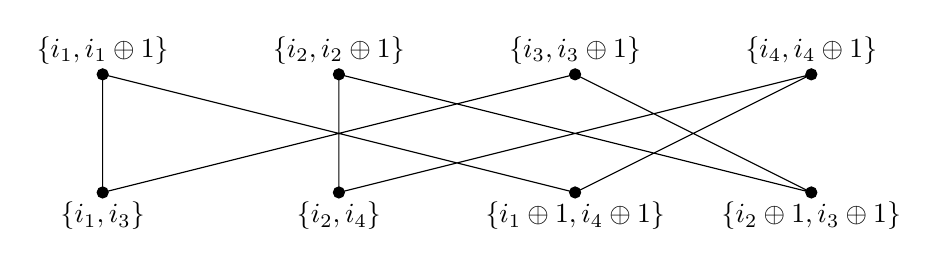
\begin{tikzpicture}[] 
\draw (0,0) -- (0,1.5) -- (6,0) -- (9,1.5) -- (3,0) -- (3,1.5) --(9,0) -- (6,1.5) -- cycle;
  \filldraw 
  (0,0) circle (2pt) node[align=left,   below] {$\edg{i_1}{i_3}$} 
  (3,0) circle (2pt) node[align=center, below] {$\edg{i_2}{i_4}$}    
  (6,0) circle (2pt) node[align=center, below] {$\edg{i_1\piu 1}{i_4\piu 1}$}   
  (9,0) circle (2pt) node[align=center, below] {$\edg{i_2\piu 1}{i_3\piu 1}$}   
  
    (0,1.5) circle (2pt) node[align=left,   above] {$\edg{i_1}{i_1\piu 1}$} 
    (3,1.5) circle (2pt) node[align=center, above] {$\edg{i_2}{i_2\piu 1}$}    
    (6,1.5) circle (2pt) node[align=center, above] {$\edg{i_3}{i_3\piu 1}$}   
    (9,1.5) circle (2pt) node[align=center, above] {$\edg{i_4}{i_4\piu 1}$}  ;
\end{tikzpicture}

\end{center}

The cycle is the disjoint union of two perfect matchings. 
From each one of them we can obtain the functions 
$\falpha()$, $\fbeta()$, $\fgamma()$, $\fdelta()$.
We adopt the convention to use the matching that contains the edge $e_1 e'_1$, where, w.l.o.g., $i_1\in e'_1$. In the example above, the matching is
\[
%\edg{i_1}{i_1\piu 1} \leftrightarrow \edg{i_1}{i_3}, \quad \edg{i_2}{i_2\piu 1} \leftrightarrow \edg{i_2}{i_4}, \quad \edg{i_3}{i_3\piu 1} \leftrightarrow \edg{i_2\piu 1}{i_3\piu 1}, \quad \edg{i_4}{i_4\piu 1} \leftrightarrow \edg{i_1\piu 1}{i_4\piu 1}
e_1 \leftrightarrow \edg{i_1}{i_3}, \quad e_2 \leftrightarrow \edg{i_2}{i_4}, \quad e_3 \leftrightarrow \edg{i_2\piu 1}{i_3\piu 1}, \quad e_4 \leftrightarrow \edg{i_1\piu 1}{i_4\piu 1}
\]
From each edge of the matching we derive either a $\tau^+$ or a $\tau^-$ expression as follows. Assume the edge is $e_x e'$, with $x\in \{1,2,3,4\}$. If $e' = \edg{i_x}{i_y}$ then
\[
c(e_x) - c(e') = c(i_x, i_x\piu 1) - c(i_x,i_y)= c(i_x, i_x\piu 1) - c(i_x,(i_y\meno 1)\piu 1) = \tau^{+}(i_x,i_y\meno 1).
\]
Otherwise, it is $e' = \edg{i_x\piu 1}{i_y}$ and 
\[
c(e_x) - c(e') = c(i_x, i_x\piu 1) - c(i_x\piu 1,i_y)= c(i_x\piu 1, i_x) - c(i_x\piu 1,(i_y\piu 1)\meno 1) = \tau^{-}(i_x\piu 1,i_y\piu 1).
\]
The sum of these values, for $x=1,2,3,4$, is then the cost of the move. For instance, in the move  above it is
\[
\Delta_r(i_1,i_2,i_3,i_4) = \tau^{+}(i_1,i_3\meno 1) + \tau^{+}(i_2,i_4\meno 1)+\tau^{-}(i_3\piu 1,i_2\piu 2)+\tau^{-}(i_4\piu 1,i_1\piu 2).
\]
Let us call $A_1,\ldots,A_4$ the four addends of the sum thus obtained (e.g., $A_1=\tau^{+}(i_1,i_3\meno 1)$, etc.) It remains to show that $A_1,\ldots,A_4$ can always be rearranged so as all four type of indices appear in the first two (which implies that they also appear  in the second two).


For $x\in \{1,2,3,4\}$ let us call a ``type-$x$ addend''
an addend in which one of the two arguments is 
either $i_x$, $i_x\meno 1$, $i_x\piu 1$ or $i_x\piu 2$.
Notice that each addend is  type-$x$  and  type-$y$ for some $x\ne y$ and that there are exactly two type-$x$ addends for each 
$x\in \{1,2,3,4\}$.
Assume $A_1$ is type-$a$ and type-$b$.
There remain three addends, and two of them are not type-$a$ or $a$ would be overrepresented. Furthermore, 
these two cannot both be type-$b$ or $b$ would be overrepresented. So there is an addend which is neither type-$a$ nor type-$b$. Swap that addend with $A_2$. Then the first two addends now range over all four indices. By reading the order in which the various types of indices appear in $A_1$ and $A_2$ we get the permutation $\pi$ of the theorem statement. Similarly, we get $\sigma$ from $A_3$ and $A_4$.
\end{proof}

In the above example, $A_1$ is type-$1$ and type-$3$, while $A_2$ is type-$2$ and type-$4$. The permutations $\pi$ and $\sigma$  are $\pi=(1,3,2,4)$ and $\sigma=(3,2,4,1)$. Furthermore,
\begin{enumerate}
\item $\falpha(x,y):=\tau^{+}(x,y\meno 1)$, with domain $\selection_{13}$
\item $\fbeta(x,y):=\tau^{+}(x,y\meno 1)$, with domain $\selection_{24}$
\item $\fgamma(x,y):=\tau^{-}(x\piu 1,y\piu 2)$, with domain $\selection_{32}$
\item $\fdelta(x,y):=\tau^{-}(x\piu 1,y\piu 2)$, with domain $\selection_{41}$
\end{enumerate}

Notice how the theorem implies that each function $f^i(x,y)$ is either a $\tau^+$ or a $\tau^-$ in which each argument is offset by 
a constant in $\{-1,0,1,2\}$.
By using Theorem \ref{teo:decom}, we can give the functions
$$\falpha,\ldots,\fdelta$$ and the permutations $\pi$ and $\sigma$ such that
$\Delta_r(i_1,i_2,i_3,i_4) = \falpha(i_{\pi(1)},i_{\pi(2)}) + \fbeta(i_{\pi(3)},i_{\pi(4)}) + \fgamma(i_{\sigma(1)},i_{\sigma(2)}) + \fdelta(i_{\sigma(3)},i_{\sigma(4)})$
for the representatives of all orbits, as reported in Table \ref{tab:f1f4}.  We recall that the permutations define also the domains of the functions $\falpha,\ldots,\fdelta$, which are, respectively, $\selection_{\pi(1)\pi(2)}$, 
$\selection_{\pi(3)\pi(4)}$, $\selection_{\sigma(1)\sigma(2)}$ and $\selection_{\sigma(3)\sigma(4)}$. 
(For a list of the inserted edges of each scheme, look at Fig. \ref{fig:orbits4}. For simplicity in checking the table 
vs the figure, we have called $i,j,k,h$ the elements that will occupy, respectively, positions $1,2,3,4$ in the selection. That is $S_{13}=\{(i,k) : \exists
 i_2,i_4 \textrm{ with } (i,i_2,k,i_4)\in \selection\}$, $S_{42}=\{(h,j) :
\exists i_1,i_3 \textrm{ with } (i_1,j,i_3,h)\in \selection\}$, etc.).

\begin{table}[h]
{%\footnotesize
	\small
\begin{center}
\begin{tabular}{|c|c|c|l|l|l|l|}
\hline  

$r$ & $\pi$ & $\sigma$ & \qquad $\falpha1()$  & \qquad\ $\fbeta()$ & \qquad\ $\fgamma()$ & \qquad\ $\fdelta()$ \\
\hline  
$\rq{1}$  &  $(1,2,4,3)$ & $(3,1,2,4)$ & $\tau^+(i,j\meno 1)$ & $\tau^-(h\piu 1,k\piu 2)$ & $\tau^+(k,i)$ & $\tau^-(j\piu 1,h\piu 1)$ \\ 
\hline  
$\rq{2}$   & $(1,2,3,4)$ & $(2,1,4,3)$ & $\tau^+(i,j\meno 1)$ & $\tau^+(k,h\meno 1)$ & $\tau^-(j\piu 1,i\piu 2)$  &  $\tau^-(h\piu 1,k\piu 2)$\\ 
\hline  
$\rq{3}$ & $(1,2,3,4)$ & $(4,1,2,3)$ & $\tau^+(i,j\meno 1)$ & $\tau^+(k,h)$ & $\tau^+(h,i)$ &  $\tau^-(j\piu 1,k\piu 2)$ \\ 
\hline 
$\rq{4}$ & $(1,2,4,3)$ & $(3,1,2,4)$ &$ \tau^+(i,j\meno 1)$ & $\tau^+(h,k\meno 1)$ & $\tau^-(k\piu 1,i\piu 2)$ & $\tau^-(j\piu 1,h\piu 2)$ \\ 
\hline 
$\rq{5}$ & $(1,2,4,3)$ & $(3,1,2,4)$ & $\tau^+(i,j\meno 1)$ & $\tau^-(h\piu 1,k\piu 1)$  & $\tau^-(k\piu 1,i\piu 2)$ & $\tau^-(j\piu 1,h\piu 1)$ \\ 
  \hline 
$\rq{10}$  & $(1,3,2,4)$ & $(3,1,4,2)$ & $\tau^+(i,k\meno 1)$ & $\tau^+(j,h)$ & $\tau^-(k\piu 1,i\piu 2)$ & $\tau^+(h,j)$ \\   
 \hline 
$\rq{25}$  & $(1,3,2,4)$ & $(3,1,4,2)$  & $\tau^+(i,k)$ & $\tau^+(j,h)$  &$\tau^+(k,i)$  & $\tau^+(h,j)$ \\   

\hline 
\end{tabular} 
\end{center}
}
\caption{Expressing $\Delta_r(i,j,k,h)$ as a sum $\falpha()+\fbeta()+\fgamma()+\fdelta()$}
\label{tab:f1f4}
\end{table}


\paragraph{A first procedure to find the best selection.}



The two-parameter functions $\falpha, \ldots,\fdelta$
can be used to  quickly discard from consideration all selections such that no two of the indices give a sufficiently large contribution to the total. Better said, we keep in consideration only candidate 4-tples for which at least one contribution of two indices is large enough.
Assume we want to find the best selection
and we currently have a selection $S^*=(\bar v_1,\bar v_2, \bar v_3,\bar v_4)$ of value $V:=\Delta_r(S^*)$ (the current ``champion'').
We make the trivial observation that for a selection
$(i_1,i_2,i_3,i_4)$ to beat $S^*$ it must be
{\small
\beq
\left(\falpha(i_{\pi(1)},i_{\pi(2)})  > \frac{V}{4} \right) \lor
\left(\fbeta(i_{\pi(3)},i_{\pi(4)})> \frac{V}{4} \right) \lor
\left(\fgamma(i_{\sigma(1)},i_{\sigma(2)})> \frac{V}{4}\right) \lor
\left(\fdelta(i_{\sigma(3)},i_{\sigma(4)}) > \frac{V}{4} \right)
\label{cond:or4}
\eeq
}

\newcommand{\basic}{{\sc BasicSmartForce}}
These are not exclusive, but possibly overlapping conditions.


Let us start by sketching a first implementation of
an algorithm for finding the best selection, based
on the approach we used for \opt{3}. We call
this approach \basic. Although this implementation is already effective and experimentally better than $O(n^3)$, we will soon describe an improvement which behaves even better (see the computational results section). 
%(*** o lasciare perdere del tutto la versione basic e andare subito con quella che funziona meglio?? ***)

\floatname{algorithm}{Procedure}
\begin{algorithm}[tb]
	\caption{\label{alg:4optimize}
		{\basic} $(r)$
		\INPUT{reinsertion scheme $r\in\{{\cal O}_1,\ldots,{\cal O}_7\}$}
		\LOCAL{heaps $H^1,\ldots,H^4$}
	}
	\begin{quote}
		\noindent\\
		\mbox{\ }1.\hspace{2mm}
		Let $\pi$ and $\sigma$ be the permutations corresponding to $r$ in Theorem \ref{teo:decom};\\
		\mbox{\ }2.\hspace{2mm}
		$H^1\leftarrow \texttt{buildHeap}(\pi(1),\pi(2), \falpha())$;\\
		\mbox{\ }3.\hspace{2mm}
		$\texttt{useHeap}(H^1,\pi(3),\pi(4))$;\\
		\mbox{\ }4.\hspace{2mm}
		$H^2\leftarrow \texttt{buildHeap}(\pi(3),\pi(4), \fbeta())$;\\
		\mbox{\ }5.\hspace{2mm}
		$\texttt{useHeap}(H^2,\pi(1),\pi(2))$;\\
		\mbox{\ }6.\hspace{2mm}
		$H^3\leftarrow \texttt{buildHeap}(\sigma(1),\sigma(2), \fgamma())$;\\
		\mbox{\ }2.\hspace{2mm}
		$\texttt{useHeap}(H^3,\sigma(1),\sigma(2))$;\\
		\mbox{\ }8.\hspace{2mm}
		$H^4\leftarrow \texttt{buildHeap}(\sigma(3),\sigma(4), \fgamma())$;\\
		\mbox{\ }9.\hspace{2mm}
		$\texttt{useHeap}(H^4,\sigma(3),\sigma(4))$;
	\end{quote}
\end{algorithm}


\basic\ is a four-phase algorithm (see Procedure \ref{alg:4optimize}). For $j=1,\ldots,4$, in the $j$-th phase, we  restrict our search to the selections $(i_1,i_2,i_3,i_4)$ which satisfy the $j$-th condition of \pref{cond:or4}. We   enumerate such selections  {\em from the most promising to the least promising}, stopping as soon as we realize that no selection of the phase has still the possibility of being the best selection overall.
To perform this  search, we use four {\em max-heaps}.
A heap is perfect  for taking the highest-valued elements 
from a set, in decreasing order. It  can be built in linear time with respect to the number of its elements and has the property that the largest element
can be extracted in logarithmic time, while still leaving a heap.
The heap is implemented by an array $H$ with three fields; $\texttt{x}$ and $\texttt{y}$, which represent two indices of a selection and $\texttt{val}$ which is a numerical value, i.e., the key to sort the heap.
By using the standard implementation of a heap \cite{cormen}, the array corresponds to a binary tree, whose nodes are stored in consecutive entries from $1$ to $\HSIZE$. The left son of node $H[t]$ is $H[2t]$, while the right son is $H[2t+1]$. The father of node $H[t]$ is $H[t.\textrm{div}.2]$. A max-heap is such that
the key of each node $H[t]$ is the largest among all the keys of the subtree rooted at $H[{t}]$.
%A call of $\texttt{heapify}(H,t)$ enforces this property for the whole subtree rooted at $H[t]$.


\floatname{algorithm}{Procedure}
\begin{algorithm}[t]
	\caption{\label{alg:buildheap}
		%\index{{\em TryOPTvalue}} 
		{\sc BuildHeap} $(a,b,f())$
		\INPUT{integers $a,b\in\{1,2,3,4\}$, function $f()$}
		\OUTPUT{Heap $H$}
	}
	\begin{quote}
		\noindent\\
		\mbox{\ }1.\hspace{2mm}
		$c \leftarrow 0$;\\
		\mbox{\ }2.\hspace{2mm}
		\FOR $(x,y)\in \selection_{a,b}$ \\ %\DO\\
		\mbox{\ }3.\hspace{8mm}
		\IF $\big(f(x,y)>V/4\big)$ \THEN\\ 
		\mbox{\ }4.\hspace{14mm}
		$c \leftarrow c+1$;\\
		\mbox{\ }5.\hspace{14mm}
		$H[c].\texttt{x} \leftarrow x$; \\
		\mbox{\ }6.\hspace{14mm}
		$H[c].\texttt{y} \leftarrow y$;\\
		\mbox{\ }7.\hspace{14mm}
		$H[c].\texttt{val} \leftarrow f(x,y)$;\\
		\mbox{\ }8.\hspace{2mm}
		$\HSIZE\leftarrow c$;\\
	\mbox{\ }9.\hspace{2mm}
		\FOR $t \leftarrow \lfloor \frac{\HSIZE}{2} \rfloor,\ldots,2,1$  \comment{turns the array into a heap}\\ %\DO
		10.\hspace{8mm}
		$\texttt{heapify}(H,t)$;\\
		11.\hspace{2mm}
		\RETURN $H$
	\end{quote}
\end{algorithm}

In phase 1 of \basic, we build a max-heap $H^{\ffalpha}$ (see Procedure \ref{alg:buildheap} {\sc BuildHeap}), 
sorted according to the  value of $\falpha$, in which
we put each triple
$(x,y,\falpha(x,y))$ such that
$(x,y)\in \selection_{\pi(1)\pi(2)}$ and
$\falpha(x,y)>V/4$. This is done
by calling {\sc BuildHeap}($\pi(1), \pi(2), \falpha$).
% If $H^{\ffalpha}$ has $L$ elements,  building the heap has cost $O(L)$, and   extracting the element of maximum $\falpha()$ value, while keeping the heap structure, has cost $O(\log L)$.
We then start extracting the elements from $H^{\ffalpha}$. Let us denote
by $(x[j],y[j],\falpha(x[j],y[j]))$ the $j$-th element extracted.
Heuristically,  $x[1]$ and $y[1]$ are  values that the pair of indices $i_{\pi(1)}$ and $i_{\pi(2)}$ would likely take in a \bimp\ selection, since they give the largest possible contribution, as far as $\falpha$ is concerned, to the move value \pref{eq:abcd}.
We  keep extracting the maximum 
$(x[j],y[j],\falpha(x[j],y[j]))$ from the heap as long as
$\falpha(x[j],y[j])>V/4$. This does not mean that we will extract all the elements of $H^{\ffalpha}$, since the value of $V$ could increase during the search and hence the extractions might terminate before the heap is empty.

Each time we extract the heap maximum,  we have that $x[j]$ and $y[j]$ are two possible indices out of four for a candidate selection to beat $S^*$. With a quadratic-time scan,
corresponding to a call of Procedure {\sc UseHeap}($H^{\ffalpha},\pi(3),\pi(4)$) (Procedure \ref{alg:useheap}), 
 we  search the two missing indices and see if we get a better selection than $S^*$ (in which case we update $V$ and $S^*$). 
For instance, if $\pi=(1,3,2,4)$,  we would run a for-cycle with $i_2$ ranging from $x[j]\piu 2$ to $y[j] \meno 2$ and $i_4$ ranging from $y[j] \piu 2$ to $\bar n - {\cal P}(x[j] = 0)$, checking each time if
$(x[j],i_2,y[j],i_4)$ is a better selection than $S^*$. Whenever this is the case, we update $S^*$. Notice that we also update $V$ so that the 
number of elements still in the heap for which $\falpha(x,y)>V/4$ may 
decrease considerably. 

\floatname{algorithm}{Procedure}
\begin{algorithm}[t]
	\caption{\label{alg:useheap}
		{\sc UseHeap} $(H,c,d)$
		%\INPUT{heap $H$, permutation $\tau$, integer $a,b\in\{1,2,3,4\}$}
		\INPUT{heap $H$, integers $c,d\in\{1,2,3,4\}$}}
	\begin{quote}
		\noindent\\
		\mbox{\ }1.\hspace{2mm}
		\WHILE $\big(H[1].\texttt{val} > V/4\big)$ \\ %\DO\\
		\mbox{\ }2.\hspace{8mm}
		$(x,y) \leftarrow \texttt{extractMax}(H)$; \\
		\mbox{\ }3.\hspace{8mm}
		\FOR $z\in\textrm { range of } i_{c}\textrm{ given } x,y$\\ % \DO\\
		\mbox{\ }4.\hspace{14mm}
		\FOR $w\in\textrm { range of } i_{d}\textrm{ given } x,y,z$ \\ %\DO\\
		\mbox{\ }5.\hspace{20mm}
		let $(i_1,i_2,i_3,i_4)$ be the selection corresponding to $\{x,y,z,w\}$;\\ 
		\mbox{\ }6.\hspace{20mm}
		\IF $(\Delta(i_1,i_2,i_3,i_4)>V)$ \THEN \comment{update global optimum}\\ 
		\mbox{\ }7.\hspace{26mm}
		$S^* \leftarrow (i_1,i_2,i_3,i_4)$;\\
		\mbox{\ }8.\hspace{26mm}
		$V \leftarrow \Delta(i_1,i_2,i_3,i_4)$;
	\end{quote}
\end{algorithm}



After this phase of probing the heap $H^{\ffalpha}$, we run three analogous phases, for $i=2,3,4$, in which we probe a heap $H^i$ containing all the
triples $(x,y,f_r^i)$ for which  $(x,y)$ is in the domain of $f_r^i$ and  and 
$f_r^i(x,y)>V/4$.
% For each element $(x[j],y[j])$ extracted from the heap, we look for the missing index $i_{\pi(1)}$. For instance, if $\pi=(1,2,3)$, the missing index would be $i_1$ and would range
%from $\PP(y[j]=\bar n)$ to $x[j]- 2$. 
Notice that the
value $V$ determining which  elements belong to   $H^i$
is the value of the current best solution, i.e., it is not the value that $V$ had at the start of the previous phase, but the value it had at its end, and gets updated each time a new best is found.

Say that, initially, the heaps have overall $L$ elements and then $M$ elements are extracted from them. Then
the cost of the procedure is $O(n^2 + L + M (n^2 + \log L))$.
Worst-case, this  is $O(n^4)$ like complete enumeration but, as
we will show in our computational experiments, it is 
{\em much} smaller in practice. 
This is because the quadruples which are indeed evaluated for
possibly becoming the best selection have a much bigger probability
of being good than a generic quadruple, since two of the four indices are
guaranteed to help the value of the move considerably.


\floatname{algorithm}{Procedure}
\begin{algorithm}[tb]
	\caption{\label{alg:find4}
		%\index{{\em TryOPTvalue}} 
		{\sc Find\opt{4}move}}
	\begin{quote}
		\noindent\\
		\mbox{\ }1.\hspace{2mm}
		$S^* \leftarrow {\tt undef}$; $\quad V\leftarrow 0$;\\
		\mbox{\ }2.\hspace{2mm}
		\FOR $i\leftarrow 1,\ldots 7$ \\%\DO\\
		\mbox{\ }3.\hspace{8mm}
		\FOR $r\in {\cal O}_{i}$ \\ %\DO\\
		\mbox{\ }4.\hspace{14mm}
		\basic$(r)$;\\
		\mbox{\ }5.\hspace{2mm}
		\IF  $(V=0)$  \THEN \\
		\mbox{\ }6.\hspace{8mm}
		\RETURN(``There are no improving moves'');\\ 
		\mbox{\ }7.\hspace{2mm}
		\ELSE\\
		\mbox{\ }8.\hspace{8mm}
		\RETURN move $S^*$ of value $V$;
	\end{quote}
\end{algorithm}


At top level, we have the  procedure {\sc Find\opt{4}move} (Procedure \ref{alg:find4}). Notice that we are calling the  reinsertion schemes in a precise order. This is somewhat arbitrary, since any other ordering would have been also valid. In the computational experiments we have considered other orders and found out that the running times are pretty much independent on the ordering chosen. In practice, we suggest to randomize the order in which the reinsertion schemes are considered, since there is no real reason to prefer an ordering over another. 
We also note that if one would choose to optimize over only some of the reinsertion schemes but not on all, it is enough to remove from the procedure the calls relative to the reinsertion schemes that one does not want to use.

For completeness, we give also the code for the  procedures 
$\textsc{Heapify}$
and $\textsc{ExtractMax}$ (Procedures \ref{alg:heapify} and \ref{alg:extract}), although they are the standard procedures for implementing heaps and can be found on any textbook on data structures. To simplify the code, we allow $H[t].\texttt{val}$ to be defined also for $t>\HSIZE$,
with value $-\infty$. The procedure $\textsc{Heapify}(H,t)$
assumes that the subtree rooted at $t$ respects the heap structure at all nodes, except, perhaps, at the root.
The procedure then adjusts the keys so that 
the subtree rooted at $t$ becomes indeed a heap. The cost of {\sc heapify} is linear in the height of the subtree. The loop of lines 11--13 in procedure $\textsc{BuildHeap}$ turns an unsorted array $H$
into a heap, working its way bottom-up, in time $O(\HSIZE)$.
The procedure {\sc ExtractMax} returns the element of maximum value of the heap (which must be in the root node, i.e., $H[1]$). It then replaces the root with a leaf and, by calling $\texttt{heapify}(H,1)$, it moves it down along the tree until the heap property is again fulfilled. The cost of this procedure is $O(\log(\HSIZE))$. 



\floatname{algorithm}{Procedure}
\begin{algorithm}[tb]
	\caption{\label{alg:heapify}
		{\sc Heapify} $(H,t)$
		\INPUT{array $H$, integer $t\in\{1,\ldots\HSIZE\}$}
	}
	\begin{quote}
		\noindent\\
		\mbox{\ }1.\hspace{2mm}
		$ls \leftarrow 2t$; \comment{left son}\\
		\mbox{\ }2.\hspace{2mm}
		$rs \leftarrow 2t+1$; \comment{right son}\\
		\mbox{\ }3.\hspace{2mm}
		\IF $\big(H[ls].\texttt{val} > H[t].\texttt{val}\big)$ \THEN\\
		\mbox{\ }4.\hspace{8mm}
		$large \leftarrow ls$;\\
		\mbox{\ }5.\hspace{2mm}
		\ELSE \\
		\mbox{\ }6.\hspace{8mm}
		$large\leftarrow t$;\\
		\mbox{\ }7.\hspace{2mm}
		\IF $ \big(H[rs].\texttt{val} > H[large].\texttt{val} \big)$ \THEN\\
		\mbox{\ }8.\hspace{8mm}
		$large \leftarrow rs$;\\
		\mbox{\ }9.\hspace{2mm}
		\IF $(large\ne t)$ \THEN\\
		10.\hspace{8mm}
		$H[t] \leftrightarrow H[large]$; \comment{swaps $H[t]$ with the largest of its sons}\\
		11.\hspace{8mm}
		$\texttt{heapify}(H,large)$;
	\end{quote}
\end{algorithm}

\floatname{algorithm}{Procedure}
\begin{algorithm}[h]
	\caption{\label{alg:extract}
		%\index{{\em TryOPTvalue}} 
		{\sc ExtractMax} $(H)$
		\INPUT{heap $H$}
		\OUTPUT{the pivot $(x,y)$ of maximum value in $H$}
	}
	\begin{quote}
		\noindent\\
		\mbox{\ }1.\hspace{2mm}
		$(x,y) \leftarrow (H[1].\texttt{x},H[1].\texttt{y})$; \comment{extracts the max element $(x,y)$}\\
		\mbox{\ }2.\hspace{2mm}
		$H[1] \leftarrow H[\HSIZE]$;\\
		\mbox{\ }3.\hspace{2mm}
		$\HSIZE \leftarrow \HSIZE -1$;\\
		\mbox{\ }4.\hspace{2mm}
		$\texttt{heapify}(H,1)$; \comment{restores the heap}\\
		\mbox{\ }5.\hspace{2mm}
		\RETURN $(x,y)$;
	\end{quote}
\end{algorithm}





\paragraph{An improved procedure to find the best selection.}

Although \basic\ proved to be already a better algorithm than the $\Theta(n^4)$ enumeration and also than the $\Theta(n^3)$ dynamic programming
procedure, we did not stop at this approach, since 
we noticed that we could do even better by grouping the four phases into two and two.

We start by replacing the condition \pref{cond:or4} with the following, stronger condition

\beq
\left(\falpha(i_{\pi(1)},i_{\pi(2)})   + \fbeta(i_{\pi(3)},i_{\pi(4)})> \frac{V}{2} \right) \lor
\left(\fgamma(i_{\sigma(1)},i_{\sigma(2)}) +
\fdelta(i_{\sigma(3)},i_{\sigma(4)}) > \frac{V}{2} \right)
\label{cond:or2}
\eeq

Just for the sake of example, assume $\pi=(1,3,2,4)$ and $\sigma=(1,4,2,3)$.
To find the optimal selection, we could run a two-phase algorithm. 
In the first phase we look for all selections $(i,j,k,h)$ such that $\falpha(i,k) + \fbeta(j,h)> \frac{V}{2}$
and then check if indeed $\Delta_r(i,j,k,h)>V$. 
In second phase, we look for all selections such that $\fgamma(i,h) + \fdelta(j,k)> \frac{V}{2}$
and then check if indeed $\Delta_r(i,j,k,h)>V$. Whenever we improve the champion, we immediately update $V$.

The procedure for each phase has in input two heaps $H'$ and $H''$ and a permutation $\phi$ of $\{1,2,3,4\}$. The heap $H'$ contains pivots in the domain $\selection_{\phi(1)\phi(2)}$ while  
$H''$ contains pivots in the domain $\selection_{\phi(3)\phi(2)}$.
Each heap corresponds to one of the addends of \pref{eq:abcd}
and is sorted according to the value
$f_H(x,y)$ of its pivots $(x,y)$ (where $f_H()$ is one of  $f_r^1,\ldots,f_r^4$).
 The goal of the phase is to form all quadruples of value $>V/2$ by picking one element from each heap. This
 is achieved by running a loop which identifies all pairs $(x,y)$, $(z,w)$ of pivots, taken from $H'$ and $H''$ respectively, such that 
$f_{H'}(x,y) + f_{H''}(z,w) > V/2$. The loop terminates as soon as the sum of the maxima of the two heaps is $\le V/2$. To perform this search effectively,  given that the maximum of $H'$ is $(x_1,y_1)$ of value $f_{H'}(x_1,y_1)$, we first extract from $H''$ all elements $(z_c,w_c)$ such that 
$f_{H'}(x_1,y_1) + f_{H''}(z_c,w_c) > V/2$.	Note that this way we have in fact created a sorted array of those elements from $H''$, i.e., $H''$ now can be replaced by an array $A''=[(z_1,w_1),\ldots,(z_Q,w_Q)]$ such that 
\[
f_{H''}(z_1,w_1) \ge \cdots \ge f_{H''}(z_Q,w_Q) > \frac{V}{2} - f_{H'}(x_1,y_1).
\]

Creating this array has cost $O(Q\log n)$. 
In a similar way, in time $O(P\log n)$ we create a sorted array $A'=[(x_1,y_1),\ldots,(x_P,y_P)]$ containing all the elements of $H'$ such that
\[
f_{H'}(x_1,y_1) \ge \cdots \ge f_{H'}(x_P,y_P) > \frac{V}{2} - f_{H''}(z_1,w_1).
\]

\floatname{algorithm}{Procedure}
\begin{algorithm}[t]
	\caption{\label{alg:combineheaps}
		{\sc CombineHeaps} $(H^0,H^1,\phi)$
		\INPUT{heaps $H^0$, $H^1$, permutation $\phi$ of $\{1,2,3,4\}$, coefficient $\alpha\in[0,1]$}
		\LOCAL{arrays $A^0$, $A^1$}}
	\begin{quote}
		\noindent\\
		\mbox{\ }1.\hspace{2mm}
		$\max^0 \leftarrow \texttt{maxval}(H^0)$; \  $\max^1 \leftarrow \texttt{maxval}(H^1)$;\\
		\mbox{\ }2.\hspace{2mm}
		\FOR $i=0,1$ \\ % \DO\\
		\mbox{\ }3.\hspace{8mm}
		$\texttt{c}\leftarrow 0$;\\
		\mbox{\ }4.\hspace{8mm}
		\WHILE ($\texttt{maxval} (H^i) + \max^{1-i} > \alpha V)$ \\ % \DO\\
		\mbox{\ }5. \hspace{14mm}
		$(x,y) \leftarrow \texttt{extractMax}(H^i)$; \\
		\mbox{\ }6.\hspace{14mm}
		\ $A^i[\texttt{c++}] \leftarrow (x,y,val)$ ;  \comment{where $val:=f_{H^i}(x,y)$}\\
		% \mbox{\ }7.\hspace{8mm}   \ENDWHILE\\
		% \mbox{\ }8.\hspace{2mm}    \ENDFOR\\
		\mbox{\ }7.\hspace{2mm}
		$p^0, p^1 \leftarrow 1;$ \comment{the part of $A^i$ still to use goes from  $p^i$ to $size(A^i)$}\\
		\mbox{\ }8.\hspace{2mm}
		\WHILE $(p^0 \le \texttt{size}(A^0)) \land (p^1 \le \texttt{size}(A^1)) \land (A^0[p^0].\texttt{val} + A^1[p^1].\texttt{val} > \alpha V)$ \\ % \DO\\
		\mbox{\ }9.\hspace{8mm}
		\IF $A^0[p^0].\texttt{val} > A^1[p^1].\texttt{val}$ \THEN $mst = 0$ \ELSE $mst=1$; \\
		10.\hspace{8mm}
		$slv \leftarrow 1 - mst$;\\
		11.\hspace{8mm}
		$\texttt{c}\leftarrow p^{slv}$;\\
		12.\hspace{8mm}
		\WHILE $(\texttt{c}\le \texttt{size}(A^{slv})) \land (
		A^{slv}[\texttt{c}].\texttt{val} + A^{mst}[p^{mst}].\texttt{val} > \alpha V)$ \\ % \DO \\
		13.\hspace{14mm}
		$(i_1, i_2, i_3, i_4) \leftarrow
		\texttt{decodeIndices}(A^{mst}[p^{mst}].(x,y),\, A^{slv}[\texttt{c}].(x,y),\, \phi)$;\\
		14.\hspace{14mm}
		\IF $(i_1,i_2,i_3,i_4) \in \selection  \land  \Delta_r( i_1,i_2,i_3,i_4 ) > V $ \THEN\\
		15.\hspace{20mm}
		$S^* \leftarrow (i_1,i_2,i_3,i_4)$;\\
		16.\hspace{20mm}
		$V \leftarrow \Delta_r(i_1,i_2,i_3,i_4)$;\\
		% 19.\hspace{14mm} \ENDIF\\
		17.\hspace{14mm}
		$\texttt{c}\leftarrow \texttt{c}+1$; \\
		% 21.\hspace{8mm} \ENDWHILE \\
		18.\hspace{8mm}
		$p^{mst} \leftarrow p^{mst}+1$; 
		% 23.\hspace{2mm} \ENDWHILE
	\end{quote}
\end{algorithm}

Now we combine elements from the first array and the second array to form all quadruples of value $>V/2$. 
For doing so we keep two pointers $a$ and $b$, one per array.
Initially $a=b=1$.
If $f_{H'}(x_a,y_a) \ge f_{H''}(z_b,w_b)$ we say that $a$ is the {\em master} and $b$ is the {\em slave}, otherwise $b$ is the {master} and $a$ the {slave}. 
We then run a double loop which ends as soon as $f_{H'}(x_a,y_a) + f_{H''}(z_b,w_b) \le V/2$. At each iteration, a pointer runs through all the elements from the slave down, as long as the sum of their values and the master's value is still $>V/2$. For example, if the master is $a$, then we would consider all elements $c=b, b+1, b+2, \ldots$ such that
 $f_{H'}(x_a,y_a) + f_{H''}(z_c,w_c) > V/2$. For each quadruple 
$(x_a,y_a,z_c,w_c)$ thus obtained we would, in time $O(1)$ sort the indices so as to obtain values $i,j,k,h$ with $i\le j \le k \le h$ and check  if indeed $(i,j,k,h)$ is a valid pure selection and $\Delta_r(i,j,k,h) > V$. In that case, we would update the current champion and its value $V$ (note that this might in turn cause an earlier termination of the loop). A more detailed description of the procedure is given in Procedure {\sc CombineHeaps} (Procedure \ref{alg:combineheaps}). For generality, in this procedure, we use a coefficient $\alpha$ to represent the fraction of $V$ that the sum of the heaps needs to achieve. Here it is $\alpha = 0.5$ but we also have a situation, described below, where we will need to set $\alpha = 1$.


Notice that once a quadruple is formed there is nothing more to do than compute its value, in time $O(1)$. If the total number of quadruples evaluated  is $L$, the complexity of the loop 8.--18. is  $O(L)$ so that, overall, the procedure takes time $O((P+Q)\log n + L)$
where $P=\texttt{size}(A^0)$ and $Q=\texttt{size}(A^1)$. As we will discuss in the section on experimental results, this procedure behaves, in practice, like $O(n^{2.5})$ 
%(*** mettere la fz giusta)


\paragraph{Perfect splits.} If we look at Table \ref{tab:f1f4} we see that there are three cases in which $\{\pi(1),\pi(2)\} = \{\sigma(1),\sigma(2)\}$
(so that, also, $\{\pi(3),\pi(4)\} = \{\sigma(3),\sigma(4)\}$). We call such a situation a {\em perfect split} of the indices, and it occurs for the orbits ${\cal O}_2$, ${\cal O}_6$ and ${\cal O}_7$ which, altogether, contain five reinsertion schemes out of 25. The reinsertion schemes with perfect split can be treated differently than the other cases, with a method that, as shown in the computational experiments section, allows us to get a further 10\% speedup over the general procedure described so far.

The key observation is that if $r$ has a perfect split we can define two functions $g_r^1()$ and $g_r^2()$ as $g_r^1=\falpha+\fgamma$ and $g_r^2=\fbeta+\fdelta$, so that 
(\ref{eq:abcd}) becomes
\[
\Delta_r(i_1,i_2,i_3,i_4) = g_r^1(i_{\pi(1)}, i_{\pi(2)})  + g_r^2(i_{\pi(3)}, i_{\pi(4)}).
\]
The domain of $g_r^1$ is $\selection_{\pi(1)\pi(2)}$ while
the domain of $g_r^2$ is $\selection_{\pi(3)\pi(4)}$. In particular, for the representatives of the above three orbits we have 

%\begin{table}[h]
\begin{center}
\begin{tabular}{|c|c|l|l|l|}
\hline  
$r$ & $\pi$ & \qquad \qquad \quad $g_r^1()$  &   \qquad \qquad \quad $g_r^2()$ \\
\hline  
$\rq{2}$   & $(1,2,3,4)$ &  $\tau^+(i,j\meno 1) + \tau^-(j\piu 1,i\piu 2)$ & $\tau^+(k,h\meno 1) + \tau^-(h\piu 1,k\piu 2)$\\ 
\hline  
$\rq{10}$  & $(1,3,2,4)$ &  $\tau^+(i,k\meno 1)+\tau^-(k\piu 1,i\piu 2)$  & $\tau^+(j,h) + \tau^+(h,j)$ \\   
 \hline 
$\rq{25}$  & $(1,3,2,4)$   & $\tau^+(i,k)+ \tau^+(k,i)$ & $\tau^+(j,h) + \tau^+(h,j)$ \\   
\hline 
\end{tabular} 
\end{center}
%\caption{Expressing $\Delta_r(i,j,k,h)$ as a sum $g_r^1()+g_r^2()$}
%\label{tab:f1f4}
%\end{table}


In order to find the best selection for a scheme with perfect split, we prepare two heaps, one sorted by the values $g_r^1()$ 
with pivots over $\selection_{\pi(1)\pi(2)}$ 
and the other by the values $g_r^2()$
with pivots over $\selection_{\pi(3)\pi(4)}$.
We  then run a unique phase of search, analogous to the
procedure {\sc CombineHeaps} (Procedure \ref{alg:combineheaps}) but with the difference that instead of computing quadruples of value $>V/2$, we compute   quadruples of value $>V$ and stop at  the first of such quadruples which turns out to be a feasible selection (since, because of the ordering of the values, it is necessarily the best selection). This is obtained by calling {\sc CombineHeaps} with $\alpha=1$.

\newcommand{\improved}{{\sc ImprovedSmartForce}}

In \improved\ (Procedure \ref{alg:4optimizeadv}) we describe the 
final version of the algorithm, which should replace \basic\ within the
overall procedure to find the best \opt{4} move (Procedure \ref{alg:find4}).



\floatname{algorithm}{Procedure}
\begin{algorithm}[tb]
	\caption{\label{alg:4optimizeadv}
		{\improved} $(r)$
		\INPUT{reinsertion scheme $r\in\{{\cal O}_1,\ldots,{\cal O}_7\}$}
		\LOCAL{heaps $H'$, $H''$}
	}
	\begin{quote}
		\noindent\\
		\mbox{\ }1.\hspace{2mm}
		Let $\pi$ and $\sigma$ be the permutations corresponding to $r$ in Theorem \ref{teo:decom};\\
		\mbox{\ }1.\hspace{2mm} 
		\IF $\pi$ and $\sigma$ are not a perfect split\\
		\mbox{\ }2.\hspace{8mm}
		$H'\leftarrow \texttt{buildHeap}(\pi(1),\pi(2), \falpha())$;\\
		\mbox{\ }2.\hspace{8mm}
		$H''\leftarrow \texttt{buildHeap}(\pi(3),\pi(4), \fbeta())$;\\
		\mbox{\ }3.\hspace{8mm}
		$\texttt{combineHeaps}(H',H'',\pi, \frac{1}{2})$;\\
		\mbox{\ }2.\hspace{8mm}
		$H'\leftarrow \texttt{buildHeap}(\sigma(1),\sigma(2), \fgamma())$;\\
		\mbox{\ }2.\hspace{8mm}
		$H''\leftarrow \texttt{buildHeap}(\sigma(3),\sigma(4), \fdelta())$;\\
		\mbox{\ }3.\hspace{8mm}
		$\texttt{combineHeaps}(H',H'',\sigma, \frac{1}{2})$;\\
		\mbox{\ }1.\hspace{2mm} 
		\ELSE  \comment{perfect split}\\
		\mbox{\ }2.\hspace{8mm}
		$H'\leftarrow \texttt{buildHeap}(\pi(1),\pi(2), \falpha() + \fgamma())$;\\
		\mbox{\ }2.\hspace{8mm}
		$H''\leftarrow \texttt{buildHeap}(\pi(3),\pi(4), \fbeta() + \fdelta())$;\\
		\mbox{\ }3.\hspace{8mm}
		$\texttt{combineHeaps}(H',H'',\pi, 1)$;\\
	\end{quote}
\end{algorithm}


\fi




\section{Methods for \opt{4} exploration in the literature}
\label{sec:literature}

In this section we describe the cubic de Berg et al. \cite{woeginger}  algorithm and the quadratic approach by Glover \cite{Glover1996}.
It must be remarked that Glover's algorithm has a very restricted scope, i.e., it 
can be applied only to 3 out of 25 reinsertion schemes, while de Berg et al. procedure is valid for
all \opt{4} moves. 


\newcommand{\costd}{\textrm{cost}_d}
\newcommand{\costc}{\textrm{cost}_c}
\newcommand{\bestA}{\textrm{bestA}}
\newcommand{\bestB}{\textrm{bestB}}
\newcommand{\bestV}{\textrm{bestV}}
\renewcommand{\myquote}[1]{``#1''}


\subsection{de Berg et al. $\Theta(n^3)$ dynamic programming approach}

For a given reinsertion scheme and selection  $(i_1,i_2,i_3,i_4)$, let  $L$ be the set of edges inserted by the scheme and  $e_k=\{i_k,i_k\piu 1\}$, for $k=1,\ldots,4$, be the edges removed.
We say that two nodes $i_s$ and $i_t$ are {\em independent} if no edge $l\in L$ is incident on both $e_s$ and $e_t$.
For instance, in Fig. \ref{fig:berg}, the nodes $a_1$ and $a_2$ are independent, while $a_1$ and $b_1$ are not, etc. 
It can be shown that, for every reinsertion 
scheme, the selection nodes
can be partitioned into two groups say $A=\{a_1, a_2\}$ and $B=\{b_1, b_2\}$
of independent nodes, and the edges $L$ can
be partitioned into $\{l_1,l_2\} \cup \{l_3,l_4\}$ in such a way that the cost of the move is 
\[
\begin{matrix*}[l]
%	c(a_1,a_1\piu 1) + c(a_2,a_2\piu 1) + 	\tilde c_1(b_1|a_1,a_2)  + 	\tilde c_2(b_2|a_1,a_2)  := \\ 
	c(a_1,a_1\piu 1) + c(a_2,a_2\piu 1) + 
	[c(b_1,b_1\piu 1) - c(l_1) - c(l_2)] + 
	[c(b_2,b_2\piu 1) - c(l_3) - c(l_4)].
\end{matrix*}
\]
Given a scheme $r$, to find the best move we can consider all possibilities for the choice of $a_1$ and $a_2$ (there are $\Theta(n^2)$ choices). For each such choice, we can then try to find the best possible completion by optimally placing the remaining two nodes $b_1$ and $b_2$ of the selection.
% in, say, positions $x$ and $y$. 
% In \cite{woeginger}, it is shown how 
This can be done via a dynamic programming procedure in time $\Theta(n)$ rather than $\Theta(n^2)$ so that the overall procedure for finding the best move for $r$ has complexity $\Theta(n^3)$.


\begin{figure}[h]
	\begin{center}
		{\footnotesize
			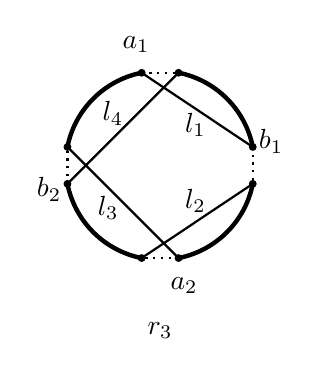
\begin{tikzpicture}[scale=0.6]
				
				\draw[ultra thick] (11.609,1.961) arc (101.25:168.75:2);
				\filldraw (13.961,0.39) circle (2pt);
				\filldraw (13.961,-0.39) circle (2pt);
				\draw [dotted,thick] (11.609,1.961) -- (12.39,1.961);
				\node at (11.492,2.55) {$a_1$};
				%				\node at (12.507,2.55) {$i_1\piu 1$};
				\draw[ultra thick] (13.961,0.39) arc (11.25:78.75:2);
				\filldraw (12.39,-1.961) circle (2pt);
				\filldraw (11.609,-1.961) circle (2pt);
				\draw [dotted,thick] (13.961,0.39) -- (13.961,-0.39);
				\node at (14.35,0.507) {$b_1$};
				\node at (12.75,0.85) {$l_1$};
				%				\node at (14.55,-0.507) {$i_2\piu 1$};
				\draw[ultra thick] (12.39,-1.961) arc (-78.75:-11.25:2);
				\filldraw (10.038,-0.39) circle (2pt);
				\filldraw (10.038,0.39) circle (2pt);
				\draw [dotted,thick] (12.39,-1.961) -- (11.609,-1.961);
				\node at (12.507,-2.55) {$a_2$};
				\node at (12.75,-0.75) {$l_2$};
				\node at (10.9,-0.9) {$l_3$};
				\node at (11.0,1.1) {$l_4$};
				%				\node at (11.492,-2.55) {$i_3\piu 1$};
				\draw[ultra thick] (10.038,-0.39) arc (-168.75:-101.25:2);
				\filldraw (11.609,1.961) circle (2pt);
				\filldraw (12.39,1.961) circle (2pt);
				\draw [dotted,thick] (10.038,-0.39) -- (10.038,0.39);
				\node at (9.649,-0.507) {$b_2$};
				%				\node at (9.449,0.507) {$i_4\piu 1$};
				\draw [thick] (11.609,1.961) -- (13.961,0.39);
				\draw [thick] (12.39,1.961) -- (10.038,-0.39);
				\draw [thick] (11.609,-1.961) -- (13.961,-0.39);
				\draw [thick] (12.39,-1.961) -- (10.038,0.39);
				
				
%				\draw[ultra thick] (17.609,1.961) arc (101.25:168.75:2);
%				\filldraw (19.961,0.39) circle (2pt);
%				\filldraw (19.961,-0.39) circle (2pt);
%				\draw [dotted,thick] (17.609,1.961) -- (18.39,1.961);
%				\node at (17.492,2.55) {$i_1$};
%				%				\node at (18.507,2.55) {$i_1\piu 1$};
%				\draw[ultra thick] (19.961,0.39) arc (11.25:78.75:2);
%				\filldraw (18.39,-1.961) circle (2pt);
%				\filldraw (17.609,-1.961) circle (2pt);
%				\draw [dotted,thick] (19.961,0.39) -- (19.961,-0.39);
%				\node at (20.35,0.507) {$i_2$};
%				%				\node at (20.55,-0.507) {$i_2\piu 1$};
%				\draw[ultra thick] (18.39,-1.961) arc (-78.75:-11.25:2);
%				\filldraw (16.038,-0.39) circle (2pt);
%				\filldraw (16.038,0.39) circle (2pt);
%				\draw [dotted,thick] (18.39,-1.961) -- (17.609,-1.961);
%				\node at (18.507,-2.55) {$i_3$};
%				%				\node at (17.492,-2.55) {$i_3\piu 1$};
%				\draw[ultra thick] (16.038,-0.39) arc (-168.75:-101.25:2);
%				\filldraw (17.609,1.961) circle (2pt);
%				\filldraw (18.39,1.961) circle (2pt);
%				\draw [dotted,thick] (16.038,-0.39) -- (16.038,0.39);
%				\node at (15.649,-0.507) {$i_4$};
%				%				\node at (15.449,0.507) {$i_4\piu 1$};
%				\draw [thick] (17.609,1.961) -- (19.961,0.39);
%				\draw [thick] (18.39,1.961) -- (17.609,-1.961);
%				\draw [thick] (16.038,-0.39) -- (18.39,-1.961);
%				\draw [thick] (19.961,-0.39) -- (16.038,0.39);
				
%				\draw[ultra thick] (2.609,-5.038) arc (101.25:168.75:2);
%				\filldraw (4.961,-6.609) circle (2pt);
%				\filldraw (4.961,-7.39) circle (2pt);
%				\draw [dotted,thick] (2.609,-5.038) -- (3.39,-5.038);
%				\node at (2.492,-4.449) {$i_1$};
%				%				\node at (3.507,-4.449) {$i_1\piu 1$};
%				\draw[ultra thick] (4.961,-6.609) arc (11.25:78.75:2);
%				\filldraw (3.39,-8.961) circle (2pt);
%				\filldraw (2.609,-8.961) circle (2pt);
%				\draw [dotted,thick] (4.961,-6.609) -- (4.961,-7.39);
%				\node at (5.35,-6.492) {$i_2$};
%				%				\node at (5.55,-7.507) {$i_2\piu 1$};
%				\draw[ultra thick] (3.39,-8.961) arc (-78.75:-11.25:2);
%				\filldraw (1.038,-7.39) circle (2pt);
%				\filldraw (1.038,-6.609) circle (2pt);
%				\draw [dotted,thick] (3.39,-8.961) -- (2.609,-8.961);
%				\node at (3.507,-9.55) {$i_3$};
%				%				\node at (2.492,-9.55) {$i_3\piu 1$};
%				\draw[ultra thick] (1.038,-7.39) arc (-168.75:-101.25:2);
%				\filldraw (2.609,-5.038) circle (2pt);
%				\filldraw (3.39,-5.038) circle (2pt);
%				\draw [dotted,thick] (1.038,-7.39) -- (1.038,-6.609);
%				\node at (0.649,-7.507) {$i_4$};
%				%				\node at (0.449,-6.492) {$i_4\piu 1$};
%				\draw [thick] (2.609,-5.038) -- (4.961,-6.609);
%				\draw [thick] (3.39,-5.038) -- (2.609,-8.961);
%				\draw [thick] (1.038,-7.39) -- (4.961,-7.39);
%				\draw [thick] (3.39,-8.961) -- (1.038,-6.609);
%				
%				
%				\draw[ultra thick] (8.609,-5.038) arc (101.25:168.75:2);
%				\filldraw (10.961,-6.609) circle (2pt);
%				\filldraw (10.961,-7.39) circle (2pt);
%				\draw [dotted,thick] (8.609,-5.038) -- (9.39,-5.038);
%				\node at (8.492,-4.449) {$i_1$};
%				%				\node at (9.507,-4.449) {$i_1\piu 1$};
%				\draw[ultra thick] (10.961,-6.609) arc (11.25:78.75:2);
%				\filldraw (9.39,-8.961) circle (2pt);
%				\filldraw (8.609,-8.961) circle (2pt);
%				\draw [dotted,thick] (10.961,-6.609) -- (10.961,-7.39);
%				\node at (11.35,-6.492) {$i_2$};
%				%				\node at (11.55,-7.507) {$i_2\piu 1$};
%				\draw[ultra thick] (9.39,-8.961) arc (-78.75:-11.25:2);
%				\filldraw (7.038,-7.39) circle (2pt);
%				\filldraw (7.038,-6.609) circle (2pt);
%				\draw [dotted,thick] (9.39,-8.961) -- (8.609,-8.961);
%				\node at (9.492,-9.55) {$i_3$};
%				%				\node at (8.492,-9.55) {$i_3\piu 1$};
%				\draw[ultra thick] (7.038,-7.39) arc (-168.75:-101.25:2);
%				\filldraw (8.609,-5.038) circle (2pt);
%				\filldraw (9.39,-5.038) circle (2pt);
%				\draw [dotted,thick] (7.038,-7.39) -- (7.038,-6.609);
%				\node at (6.649,-7.507) {$i_4$};
%				%				\node at (6.449,-6.492) {$i_4\piu 1$};
%				\draw [thick] (8.609,-5.038) -- (9.39,-8.961);
%				\draw [thick] (10.961,-7.39) -- (7.038,-7.39);
%				\draw [thick] (8.609,-8.961) -- (9.39,-5.038);
%				\draw [thick] (10.961,-6.609) -- (7.038,-6.609);
%				
%				\draw[ultra thick] (14.609,-5.038) arc (101.25:168.75:2);
%				\filldraw (16.961,-6.609) circle (2pt);
%				\filldraw (16.961,-7.39) circle (2pt);
%				\draw [dotted,thick] (14.609,-5.038) -- (15.39,-5.038);
%				\node at (14.492,-4.449) {$i_1$};
%				%				\node at (15.507,-4.449) {$i_1\piu 1$};
%				\draw[ultra thick] (16.961,-6.609) arc (11.25:78.75:2);
%				\filldraw (15.39,-8.961) circle (2pt);
%				\filldraw (14.609,-8.961) circle (2pt);
%				\draw [dotted,thick] (16.961,-6.609) -- (16.961,-7.39);
%				\node at (17.35,-6.492) {$i_2$};
%				%				\node at (17.55,-7.507) {$i_2\piu 1$};
%				\draw[ultra thick] (15.39,-8.961) arc (-78.75:-11.25:2);
%				\filldraw (13.038,-7.39) circle (2pt);
%				\filldraw (13.038,-6.609) circle (2pt);
%				\draw [dotted,thick] (15.39,-8.961) -- (14.609,-8.961);
%				\node at (15.507,-9.55) {$i_3$};
%				%				\node at (14.492,-9.55) {$i_3\piu 1$};
%				\draw[ultra thick] (13.038,-7.39) arc (-168.75:-101.25:2);
%				\filldraw (14.609,-5.038) circle (2pt);
%				\filldraw (15.39,-5.038) circle (2pt);
%				\draw [dotted,thick] (13.038,-7.39) -- (13.038,-6.609);
%				\node at (12.649,-7.507) {$i_4$};
%				%				\node at (12.449,-6.492) {$i_4\piu 1$};
%				\draw [thick] (14.609,-5.038) -- (14.609,-8.961);
%				\draw [thick] (13.038,-7.39) -- (16.961,-7.39);
%				\draw [thick] (15.39,-8.961) -- (15.39,-5.038);
%				\draw [thick] (16.961,-6.609) -- (13.038,-6.609);
				
				{\normalsize
%					\node at (0,-3.5) {$\rq{1}$};
%					\node at (6,-3.5) {$\rq{2}$};
					\node at (12,-3.5) {$\rq{3}$};
%					\node at (3,-10.5) {$\rq{5}$};
%					\node at (9,-10.5) {$\rq{10}$};
%					\node at (15,-10.5) {$\rq{25}$};
				}
				
			\end{tikzpicture}
		}
		\caption{An example reinsertion scheme for de Berg's et al. algorithm}
		\label{fig:berg}
	\end{center}
\end{figure}

Given the placement of the two fixed nodes $a_1$ and $a_2$, the value of a selection is split into three parts, i.e., a constant part $c(a_1,a_1\piu 1)+c(a_2,a_2\piu 1)$ depending only on $a_1,a_2$ plus two contributions 
\[
\tilde c_1(b_1|a_1,a_2) := c(b_1,b_1\piu 1) - c(l_1) - c(l_2)
\]
and 
\[
\tilde c_2(b_2|a_1,a_2) := c(b_2,b_2\piu 1) - c(l_3) - c(l_4)
\]
which we seek to maximize. Each of these contribution accounts for the cost of one removed edge minus the cost of two inserted edges. Since the positions $b_1$ and $b_2$ are independent,  all the inserted edges get counted exactly once.
For instance, with respect to the reinsertion scheme $r_3$ in Fig. \ref{fig:berg}, in which  $a_1=i_1$ and $a_2=i_3$,  it is
\[
\tilde c_1(b_1|a_1,a_2) = c(b_1,b_1\piu 1) - c(b_1,a_1) - c(b_1\piu 1,a_2\piu 1) 
\]
and 
\[
{\tilde c}_2(b_2|a_1,a_2) = c(b_2,b_2\piu 1) - c(b_2,a_2\piu 1) - c(b_2\piu 1,a_2).
\]
\ \\
In order to find the placement of $b_1$ and $b_2$ which maximizes $\tilde c_1(b_1|a_1,a_2)+\tilde c_1(b_2|a_1,a_2)$, we consider a general situation in which there is a range of consecutive positions $\{\min_1,\ldots, \max_1\}$ where we have to place $b_1$ and a range $\{\min_2,\ldots, \max_2\}$ for $b_2$. These ranges depend on the scheme $r$. E.g., in our example, it is $\min_1= a_1+2$, $\max_1=a_2-2$, and $\min_2 = a_2 + 2$,  $\max_2=\bar{n} - \PP{a_1=0}$. 

For $j\in \{\min_1,\ldots,\max_1\}$ let us call $V_1[j]$ the best value of a feasible partial selection $\{a_1,a_2,b_1\}$ for which $b_1\in \{\min_1, \ldots, j\}$, and let $\bestV_1[j]$ be the corresponding choice for $b_1$. 
% We also define $V_1[j]:=-\infty$ if $j\notin \{\min_1,\ldots,\max_1\}$. 
We have the general recurrence, for $\min_1 < j \le \max_1$,
\[
V_1[j] = \max\{V_1[j-1],\, {\tilde c}_1(j|a_1,a_2)\}
\]
where $\bestV_1[j]\leftarrow \bestV_1[j-1]$ if the
max is achieved by first term, and  $\bestV_1[j]\leftarrow  j$ otherwise.


Similarly, let $V_2[j]$ the best value of a feasible selection $\{a_1,a_2,b_1,b_2\}$ for which $b_2\in \{\min_2,\ldots, j\}$ and  let $\bestV_1[j]$ be the best value for $b_2$.  We have the general recurrence, for $\min_2 < j \le \max_2$,
\[
V_2[j] = \max\{V_2[j-1],\, {\tilde c}_2(j|a_1,a_2) + V_1[\min \{ j-2, \textrm{max}_1\}]\}.
\]
where $\bestV_2[j]\leftarrow \bestV_2[j-1]$ if the
max is achieved by first term, and  $\bestV_2[j]\leftarrow  j$ otherwise.

The optimal solution value for $a_1$, $a_2$ is found in $V_2[\max_2]$ and can be computed in time $\Theta(n)$ by filling the arrays $V_1[\cdot]$ and $V_2[\cdot]$. The optimal completion of $a_1, a_2$ is
$b_2:= \bestV_2[\textrm{max}_2]$ and $b_1:=\bestV_1[\min \{ b_2-2, \textrm{max}_1\}]$.


\subsection{Glover's $\Theta(n^2)$ algorithm}

In this section we briefly describe Glover's $\Theta(n^2)$ algorithm
for finding the best \opt{4} move. The algorithm works only for a restricted set of reinsertion
schemes, i.e., $r_{10}$, $r_{16}$ (orbit ${\cal O}_{6}$) and $r_{25}$ (orbit ${\cal O}_7$). For convenience, we report these orbits in Fig. \ref{fig:glover}. 

We use a different (simpler but equivalent) explanation than in Glover's paper, based
on dynamic programming. The description is recursive, but in the
implementation, by using memoization, the recursion is avoided. The
running time is $\Theta(n^2)$.

\begin{figure}[h]
	\begin{center}
		{\footnotesize
			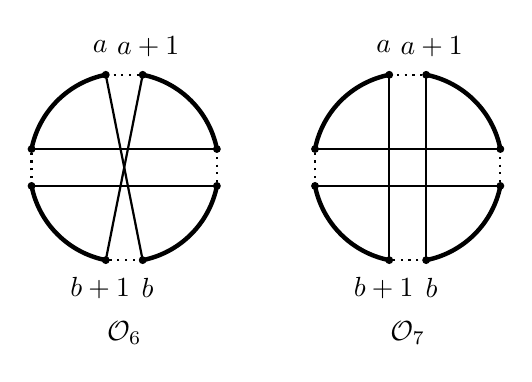
\begin{tikzpicture}[scale=0.6]
				
				\draw[ultra thick] (8.609,-5.038) arc (101.25:168.75:2);
				\filldraw (10.961,-6.609) circle (2pt);
				\filldraw (10.961,-7.39) circle (2pt);
				\draw [dotted,thick] (8.609,-5.038) -- (9.39,-5.038);
				\node at (8.492,-4.449) {$a$};
				\node at (9.507,-4.449) {$a + 1$};
				\draw[ultra thick] (10.961,-6.609) arc (11.25:78.75:2);
				\filldraw (9.39,-8.961) circle (2pt);
				\filldraw (8.609,-8.961) circle (2pt);
				\draw [dotted,thick] (10.961,-6.609) -- (10.961,-7.39);
				%	\node at (11.35,-6.492) {$i_2$};
				%				\node at (11.55,-7.507) {$i_2\piu 1$};
				\draw[ultra thick] (9.39,-8.961) arc (-78.75:-11.25:2);
				\filldraw (7.038,-7.39) circle (2pt);
				\filldraw (7.038,-6.609) circle (2pt);
				\draw [dotted,thick] (9.39,-8.961) -- (8.609,-8.961);
				\node at (9.492,-9.55) {$b$};
				\node at (8.492,-9.55) {$b + 1$};
				\draw[ultra thick] (7.038,-7.39) arc (-168.75:-101.25:2);
				\filldraw (8.609,-5.038) circle (2pt);
				\filldraw (9.39,-5.038) circle (2pt);
				\draw [dotted,thick] (7.038,-7.39) -- (7.038,-6.609);
				%	\node at (6.649,-7.507) {$i_4$};
				%				\node at (6.449,-6.492) {$i_4\piu 1$};
				\draw [thick] (8.609,-5.038) -- (9.39,-8.961);
				\draw [thick] (10.961,-7.39) -- (7.038,-7.39);
				\draw [thick] (8.609,-8.961) -- (9.39,-5.038);
				\draw [thick] (10.961,-6.609) -- (7.038,-6.609);
				
				\draw[ultra thick] (14.609,-5.038) arc (101.25:168.75:2);
				\filldraw (16.961,-6.609) circle (2pt);
				\filldraw (16.961,-7.39) circle (2pt);
				\draw [dotted,thick] (14.609,-5.038) -- (15.39,-5.038);
				\node at (14.492,-4.449) {$a$};
				\node at (15.507,-4.449) {$a+ 1$};
				\draw[ultra thick] (16.961,-6.609) arc (11.25:78.75:2);
				\filldraw (15.39,-8.961) circle (2pt);
				\filldraw (14.609,-8.961) circle (2pt);
				\draw [dotted,thick] (16.961,-6.609) -- (16.961,-7.39);
				%	\node at (17.35,-6.492) {$b$};
				%				\node at (17.55,-7.507) {$i_2\piu 1$};
				\draw[ultra thick] (15.39,-8.961) arc (-78.75:-11.25:2);
				\filldraw (13.038,-7.39) circle (2pt);
				\filldraw (13.038,-6.609) circle (2pt);
				\draw [dotted,thick] (15.39,-8.961) -- (14.609,-8.961);
				\node at (15.507,-9.55) {$b$};
				\node at (14.492,-9.55) {$b+ 1$};
				\draw[ultra thick] (13.038,-7.39) arc (-168.75:-101.25:2);
				\filldraw (14.609,-5.038) circle (2pt);
				\filldraw (15.39,-5.038) circle (2pt);
				\draw [dotted,thick] (13.038,-7.39) -- (13.038,-6.609);
				%	\node at (12.649,-7.507) {$i_4$};
				%				\node at (12.449,-6.492) {$i_4\piu 1$};
				\draw [thick] (14.609,-5.038) -- (14.609,-8.961);
				\draw [thick] (13.038,-7.39) -- (16.961,-7.39);
				\draw [thick] (15.39,-8.961) -- (15.39,-5.038);
				\draw [thick] (16.961,-6.609) -- (13.038,-6.609);
				
				{\normalsize
					\node at (9,-10.5) {${\cal O}_{6}$};
					\node at (15,-10.5) {${\cal O}_{7}$};
				}
				
			\end{tikzpicture}
		}
		\caption{Orbits for Glover's algorithm}
		\label{fig:glover}
	\end{center}
\end{figure}


\paragraph{Orbit ${\cal O}_7$.}

Orbit ${\cal O}_7 = \{r_{25}\}$ (also called the \myquote{two bridges} reinsertion scheme, because of 
its peculiar shape)  can be seen as the combination of
two independent moves of two edges each.
Each such move, let us call it $M(a,b)$, removes the edges $\edg{a}{a+1}$ and $\edg{b}{b+1}$ and
introduces $\edg{a}{b+1}$ and $\edg{a+1}{b}$, thus disconnecting the tour. Let us call the cost of this disconnecting move
\[
\costd(a,b) := c(a,a+1) + c(b,b+1) - (c(a,b+1) + c(a+1,b)).
\]



 
We define two dynamic programming tables $A[i,j]$ and $B[i,j]$, for $0\le i < j \le \bar n$. The meaning of $A$ is
$A[i,j]$=\myquote{value of the best possible move $M(a,j)$ with $a\le i$}. I.e., the move removes
 an edge $\edg{a}{a+1}$ in the interval $0,\ldots,i$ together with $\edg{j}{j+1}$. The best value for $a$ is saved in an array $\bestA[i,j]$. We have the following recursion:
\[
A[i,j] = \max\{ \costd(i,j), A[i-1,j] \}
\]
where the first case is when we remove $\edg{i}{i+1}$, while the
second case is when we do not. Base case occurs when $i=0$.

The meaning of $B$ is $B[i,j]$=\myquote{value of the best possible move $M(a,b)$ with $0\le a\le i-2$ and $i+2 \le b\le j-2$}. I.e., the move removes an edge $\edg{a}{a+1}$ to the left of $i$ (in the interval $0,\ldots,i-2$) together with an edge $\edg{b}{b+1}$ to the right of $i$ but to the left of $j$ (i.e., in the interval $i+2,\ldots,j-2$). The best value for $(a,b)$ is saved in $\bestB[i,j]$.
We have the following recursion:
\[
B[i,j] = \max\{ A[i-2,j-2], B[i,j-1] \}
\]
where the first case is when we do remove the rightmost possible arc, i.e., $\edg{j-2}{j-1}$, while the
second case is when we do not. Base case occurs when $j-2=i+2$.
When the max is the first term, $\bestB[i,j] := (\bestA[i-2,j-2], j-2)$. When
it is the second, $\bestB[i,j]:=\bestB[i,j-1]$.

At this point, we can state the whole dynamic programming algorithm,
by guessing two of the edges of the \opt{4} move, namely the
2nd $\edg{i_2}{i_2+1}$ and the 4th $\edg{i_4}{i_4+1}$ and completing in the best possible way with the 1st and 3rd. We compute $B[x,y]$ in time $O(n^2)$ and then, still in time $O(n^2)$
\[
OPT(r_{25}) := \max \{\costd(i_2,i_4) + B[i_2,i_4] : 2\le i_2 < i_4 -4 \le i_4 < \bar n \}.
\]

If $i'_2$ and $i'_4$ realize the above maximum, then the
best move is completed by setting
\[
(i'_1, i'_3) := \bestB[i'_2, i'_4].
\]

\paragraph{Orbit ${\cal O}_6$.}

Orbit ${\cal O}_6$ is made by one \myquote{crossed} bridge and one \myquote{parallel} bridge, intertwined. If the first bridge (the one indexed by $i_1$ and $i_3$) is the crossed one, we have reinsertion scheme $r_{10}$, otherwise we have $r_{16}$. The cost of 
a crossed bridge indexed by $a$ and $b$ is
\[
\costc(a,b) := c(a,a+1) + c(b,b+1) - (c(a,b) + c(a+1,b+1)).
\]


We can use a similar dynamic program as before. In the previous section, $B[x,y]$ finds the best placement of a \myquote{parallel} bridge
given $x$ and $y$, and is based on the cost $\costd$. If
we were to replace $\costd()$ with $\costc()$ in the definition of $A[,]$, then  $B[x,y]$ would find the best placement of a \myquote{crossed}
 bridge given $x$ and $y$. So let us assume that $B^c$ is the version
of $B$ using $\costc()$, while 
$B^d$ is the version
of $B$ using $\costd()$. Then
\[
OPT(r_{16}) := \max \{\costc(i_2,i_4) + B^d[i_2,i_4] : 2\le i_2 < i_4 -4 \le i_4 < \bar n \}
\]
and 
\[
OPT(r_{10}) := \max \{\costd(i_2,i_4) + B^c[i_2,i_4] : 2\le i_2 < i_4 -4 \le i_4 < \bar n \}.
\]


\bibliographystyle{plain}
\bibliography{tspbib}

\end{document}

